\documentclass{article}
\usepackage{graphicx} % Required for inserting images
\usepackage{titlesec}
\usepackage{tabularx}
\usepackage{makecell} 
\usepackage{array} 
\usepackage{enumitem}
\usepackage{changepage}  
\usepackage{geometry}
\usepackage{float}
\usepackage[none]{hyphenat}
\setcounter{secnumdepth}{4}

\titleformat{\paragraph}
{\normalfont\normalsize\bfseries}{\theparagraph}{1em}{}
\titlespacing*{\paragraph}
{0pt}{3.25ex plus 1ex minus .2ex}{1.5ex plus .2ex}

\title{\textbf{Design Document}}
\author{Armando Fiorini, Samuele Motta, Vajihe Gholami}
\date{}

\begin{document}

\maketitle
\section*{INFO}
\textbf{Deliverable}: DD\\
\textbf{Title}: Design Document\\
\textbf{Authors:} Armando Fiorini, Samuele Motta, Vajihe Gholami\\
\textbf{Version:} 0.0.0\\
\textbf{Date}: 17/12/2023\\
\textbf{Download page}: https://github.com/ArmaFio/FioriniMottaGholami\\
\newpage
\tableofcontents
\newpage

\section{Introduction}
\subsection{Purpose}
The main purpose of the present document is to support the development team in realizing the system. It provides an overall description of the adopted system architecture and a breakdown of the various components to a significant extent, also describing their interactions with each other. On top of that, the Design Document (DD) describes the implementation, integration, and testing plans which are defined keeping into account priority, required effort, and impact of the single components on the stakeholders.

\subsection{Scope}
CodeKataBattle (CKB) helps students improve their software skills through teamwork on coding challenges. It's all about learning together in a fun, competitive way. Educators create tournaments with coding exercises, and students form teams to solve them. The platform handles everything: deadlines, tests, and checking code quality. \\
Educators can also give personal feedback and scores. CKB is where educators set challenges, students solve them as teams, and everyone can see how they're doing. It handles tournaments, battles, team setups, code submissions via GitHub, live scoring, and awarding badges for achievements. \\
The system focuses on teamwork, good coding methods using tests, and a mix of competition and support. Automated tools ensure fair assessments while letting educators give helpful feedback. Badges and student profiles make it fun, encouraging everyone to participate and shine. Overall, CKB is a platform mixing learning, teamwork, competition, and skill-building in software development.

\subsection{Definitions, Acronyms, Abbreviations}
\subsubsection{Definitions}
\textbf{Educator:} A user who signs up to use the system to improve his students' programming skills can create Tournaments and badges. \\\\
\textbf{Student:} user who signs up to improve their skills, and participate in tournaments are created by the educators. \\\\
\textbf{Tournament:} coding challenge, consisting of a certain number of battles. Team: group of students, formed to join a tournament and work together to win the battles. \\\\
\textbf{Battle:} every single challenge the tournament is composed of. \\\\
\textbf{(Gamification) Badge:} achievement that is created by an educator, and can be obtained from Students satisfying the established requirements.\\

\subsubsection{Acronyms}
\begin{itemize}
    \item \textbf{CKB}: CodeKataBattle
    \item \textbf{RASD}: Requirement Analysis and Specification Document
    \item \textbf{UI}: User Interface
    \item \textbf{UML}: Unified Modelling Language
    \item \textbf{OS}: Operative System
\end{itemize}

\subsubsection{Abbreviations}
\begin{itemize}
    \item \textbf{$[Gn]$}: the n-th goal of the system.
    \item \textbf{$[Wn]$}: the n-th world phenomena.
    \item \textbf{$[SWn]$}: the n-th shared phenomena controlled by the world.
    \item \textbf{$[SMn]$}: the n-th shared phenomena controlled by the machine.
    \item \textbf{$[Dn]$}: the n-th domain assumption.
    \item \textbf{$[FRn]$}: the n-th functional requirement.
\end{itemize}

\subsection{Revision History}
\begin{itemize}
    \item Version 1.0 (January 7, 2024)
\end{itemize}


\subsection{Reference Documents}
This document is based on:
\begin{itemize}
    \item The specification of the RASD and DD assignment of the Software Engineering II course, held by Professor Matteo Rossi, Elisabetta Di Nitto, and Matteo Camilli at the Politecnico di Milano, A.Y 2023/2024; 
    \item Slides of Software Engineering 2 course on WeBeep;
\end{itemize}


\subsection{Document Structure}
Mainly the current document is divided into 4 chapters, which are:
\begin{itemize}
    \item \textbf{Introduction:} The first chapter includes the introduction which explains the purpose of the document, then, a brief recall of the concepts introduced in the RASD is given. Finally, important information for the reader is given, i.e. definitions, acronyms, synonyms, and the set of documents referenced. 
    \item \textbf{Architectural Design:} It includes a detailed description of the architecture of the system, including the high-level view of the elements, the software components of …, a description through run-time diagrams of various functionalities of the system, and, finally, an in-depth explanation of the architectural pattern used.
    \item \textbf{User Interface Design:} Provide mock-ups of the application user interfaces, with the links between them to help in understanding the flow between them. 
    \item \textbf{Requirements Traceability:} It describes the connections between the requirements defined in the RASD and the components described in the first chapter. This is used as proof that the design decisions have been taken concerning the requirements, and therefore that the designed system can fulfill the goals. 
    \item \textbf{Implementation, Integration, and Test Plan:} It describes the process of implementation, integration, and testing to which developers have to stick to produce the correct system correctly. 
    \item \textbf{Effort Spent:} Contains information about the time spent to create this document. 
    \item \textbf{References:} It contains the references to any documents and the Software used in this document. 
\end{itemize}
\section{Architectural Design}

\subsection{Overview}
This section gives an overview of the architectural elements that compose the system, their interaction, and a description of the replication mechanism chosen for the system to make it distributed.
\subsection{High-Level view}
The CodeKataBattle project follows a 3-tier architecture, segregating its functionalities into distinct layers. (Figure \ref{fig:3-tier}) The Presentation Layer handles the user interface, authentication, notifications, and badge visualization. The Application Layer contains the core logic, managing battles, tournaments, GitHub integration, score calculation, and badge generation. The Data Layer ensures data integrity and storage, interacting with the database and employing ORM for data operations. Communication between these tiers occurs through APIs or service calls. This modular structure streamlines development, fostering scalability and maintainability. The front end allows user interaction while the back end manages logic, data, and integrations, providing educators and students with a seamless platform to engage in code kata battles and tournaments, track progress, and visualize achievements through earned badges.
\begin{figure}[H]
    \centering
    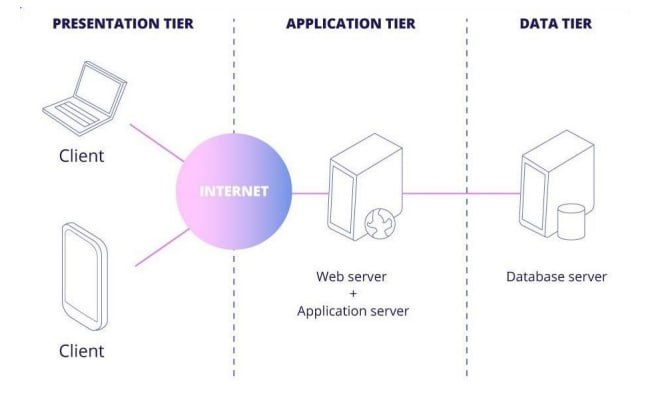
\includegraphics[width=\linewidth]{High level view.jpg}
    \caption{3-tier architecture}
    \label{fig:3-tier}
\end{figure}
\noindent
Regardless of whether the user is an educator or a student, they can access the application through either the web or mobile app, with communication between the client and server relying on various components tailored to the consumer device's type.\\
Both the web app and the mobile app communicate with the common application server: the web app will need a web server to reach this purpose through a web browser, the web server will take the web app HTTP requests and forward them to the application server, then it will return a web page as a response to the web app.\\
The application server will use HTTP protocol for communication in order to adapt to all the client types he has to interact with.\\
The application server has to be put in communication with an e-mail provider, to manage confirmation emails for registrations, GitHub, which the system has to use during battles to create the Repository with the CodeKata and to take the participants' solutions, and, which is a code static analysis tool, used to evaluate the code of all the teams that are competing in battles.\\
All the data of the System, regarding profiles tournaments battles, and gamification badges, created from the web or mobile application, will be stored in a unique DBMS, which is shared between Educators and Students and can be written and read by the application server.
The web server is not directly connected with the DBMS: in fact, it cannot satisfy the client requests by himself, all the web app requests are handled by the application server.


\begin{figure}[H]
    \centering
    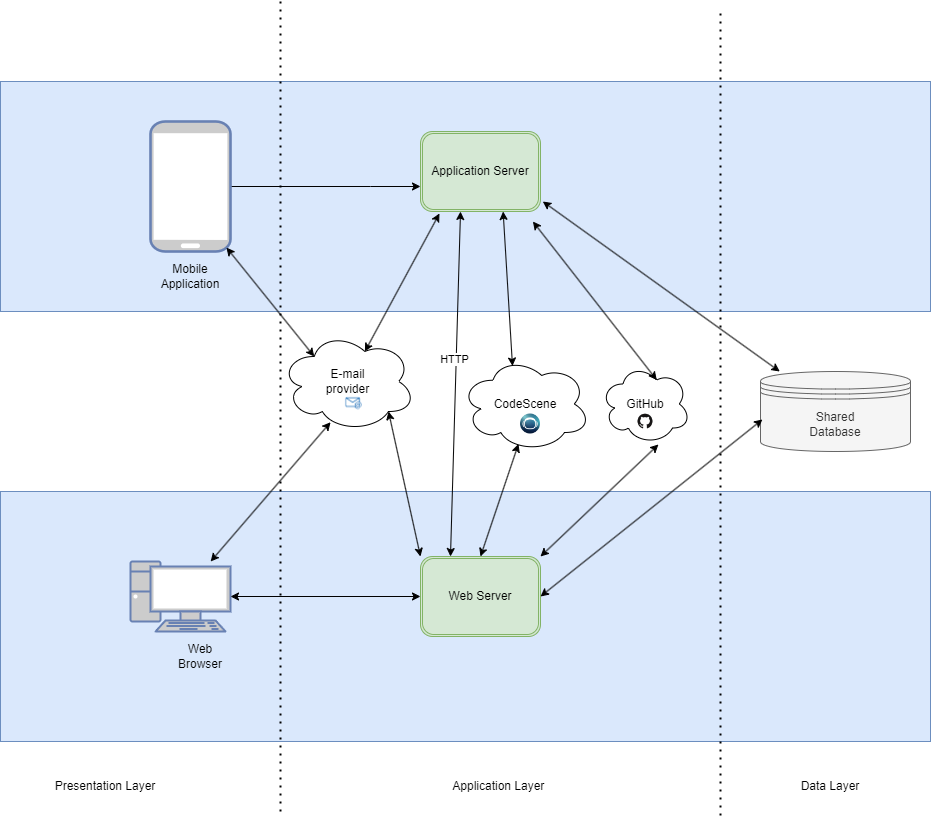
\includegraphics[width=\linewidth]{HighLevelSystemArchitecture.png}
    \caption{High-Level System Architecture}
\end{figure}
\newpage

\subsection{Component view}
This section describes the system's component diagram, outlining all internal and external elements.

\begin{figure}[H]
    \centering
    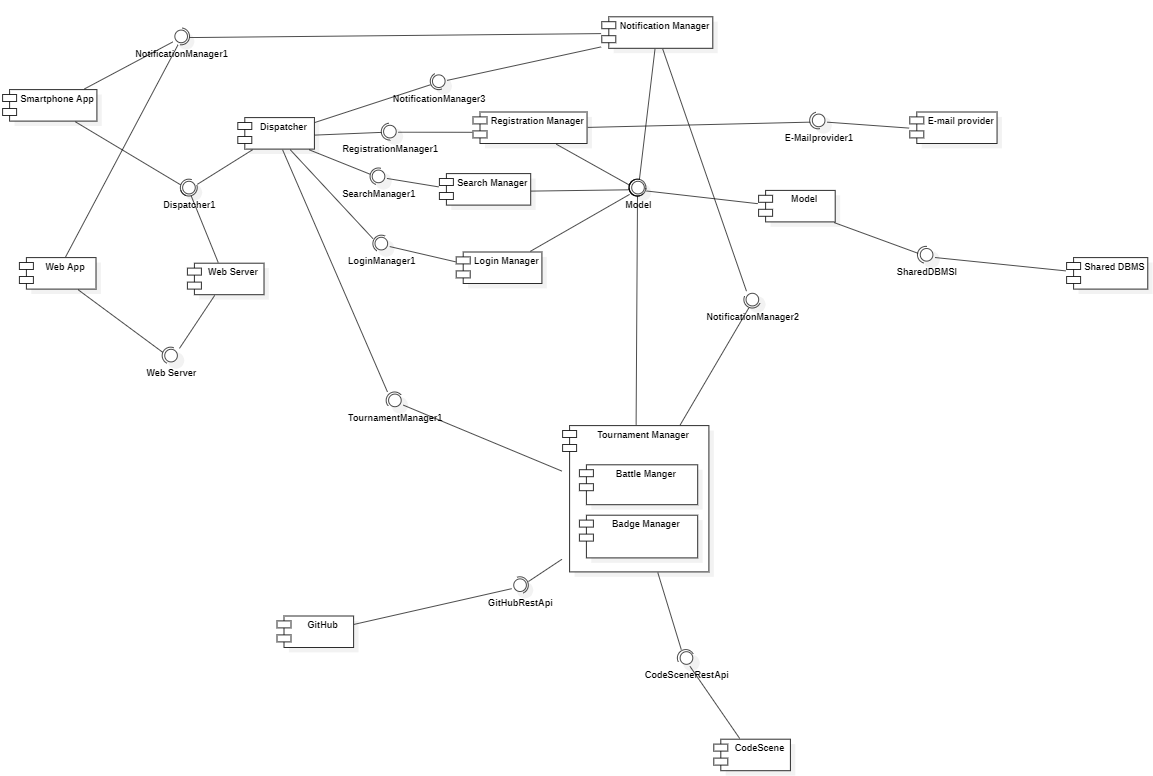
\includegraphics[width=\linewidth]{Component diagram.png}
    \caption{Component Diagram}
\end{figure}
\begin{itemize}
    \item \textbf{Smartphone App}: it's the application that needs to be installed on a mobile device to 
    get access to the system.\\
    The Smartphone App can communicate directly with the application server: every request made by it is sent to the dispatcher, which will return the corresponding answer.
    \item \textbf{Web App}: it's the web version of the CKB Application, which can be accessed from an internet browser: it's connected to the application server through the web server which handles the requests before forwarding them to the dispatcher.
    \item \textbf{Web Server}: it's the component that connects the Web Application with the Application Server: the Web Server acts as a link between the Web Application and the Dispatcher, to which it forwards all the requests made by the first one, receiving the corresponding answers. 
    \item \textbf{Dispatcher}: the Dispatcher receives all the requests from the Smartphone App and the web server and manages them contacting the corresponding component: when the request has been correctly processed it returns the answer to the caller.
    \item \textbf{Login Manager}: this component handles all the login requests made by users of the system: it checks the credentials and, if they are correct, sends the Dispatcher the corresponding account data to fill the user's dashboard.
    \item \textbf{Registration Manager}: this component handles the registration procedures for new users of the system: it checks the availability of the credentials they want to use and if they are available it manages the creation of the new account and sends to the Dispatcher the confirmation of the completion of the registration.
    This component interacts with the \textbf{E-mail provider} to handle the procedure of the user's e-mail confirmation, when a new account is being created.
    \item \textbf{Tournament Manager}: this component handles the management of all concerning the tournament creation, conduction, and closure.\\
    The tournament manager has two subcomponents used to handle some specific aspects of the tournament: in particular the creation and management of the single battles are handled by the \textbf{Battle Manager}, which also uses the connections with \textbf{GitHub} and \textbf{CodeScene} to create the repository for the battle and evaluate the students' solutions for the battle, the creation and assignments of the badges are instead handled by the \textbf{Badge Manager}.
    \item \textbf{Search Manager}: the search manager manages all the requests of account searching and visualizing: it takes from the database the requested accounts or list and returns them to the dispatcher to be shown to the user.
    \item \textbf{Notification Manager}: the notification manager manages the creation storing and visualization of notifications: it is directly linked to the Tournament Manager which uses its interface when a notification about a tournament itself has to be sent to one or more users.\\
    This component is also connected to the model and dispatcher to manage the notifications visualization requests: when a user accesses the notifications section in the mobile/web application, a request for the list of pending notifications is sent to the system and forwarded by the dispatcher to the notification manager which takes the data from the DBMS
    \item \textbf{Model}: the Model is the component of the system that contains all the representations of entities involved in the system: when some data has to be taken from the DBMS the task is assigned to the model which stores them in the appropriate data structure.
    The model also offers the methods that are necessary to modify, manipulate, and interact with the entities of the system.
    It's the only component that can directly interact with the DBMS.
    \item \textbf{Shared DBMS}: the DBMS is used to store all the data regarding all the tournaments, battles, and users of the system.
    This component solves queries and returns the data to the model to be stored in the system through the data structures provided by the model.
\end{itemize}
\newpage
\subsection{Deployment view}
This chapter provides insights into the deployment view of CKB, detailed in \textbf{Figure 3}. Within this view, we delve into the execution environment of the system, elucidating the physical distribution of the hardware components responsible for executing the software that forms the application.
\begin{figure}[H]
    \centering
    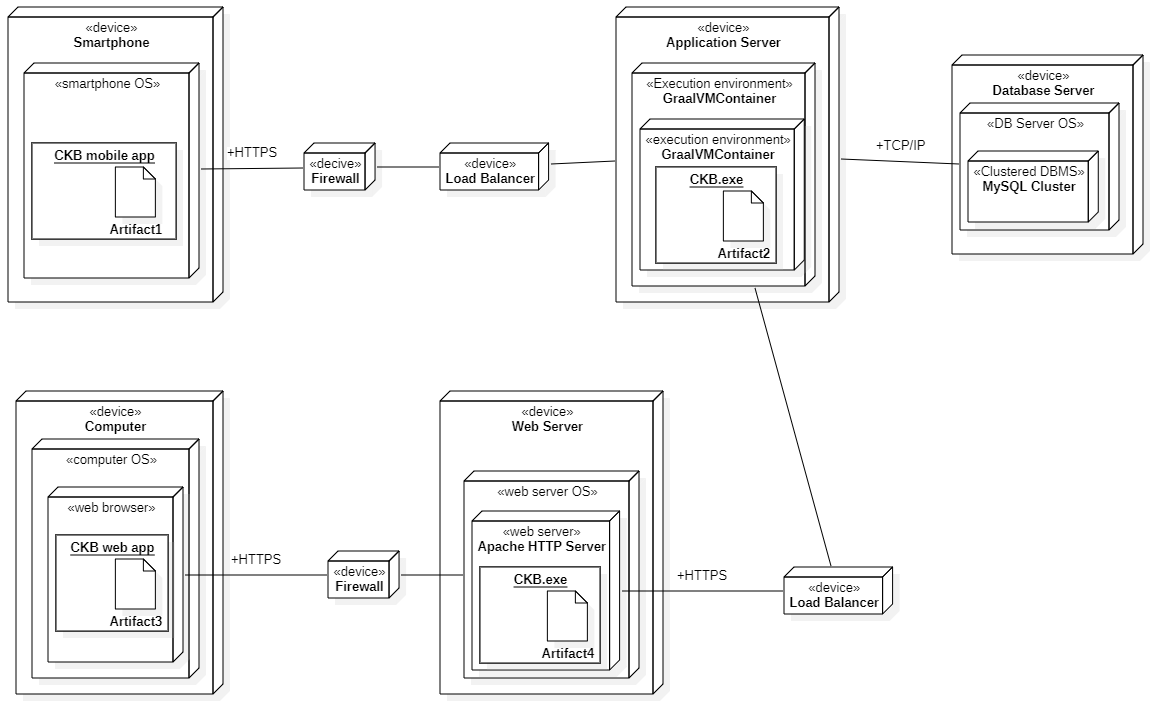
\includegraphics[width=\linewidth]{deployment diagram.png}
    \caption{System Deployment View}
\end{figure}
\noindent
Additional intricacies about the elements depicted in the graph are elaborated in the following sections.
\begin{itemize}
    \item \textbf{Smartphone} \\
    The smartphone, acting as a client, can install the CKB app. Communication between the software and the system occurs through HTTPS requests, which are directly transmitted to the Application Server without passing through the Web Server.
    \item \textbf{Computer} \\
    The computer is a standard device with internet access through a web browser. Users will utilize the web browser to explore the internet and locate the CKB webpage. Via an HTTPS request, the web server accesses the Application Server, forwarding the request to provide the required service.
    \item \textbf{Firewall} \\
    The firewall, positioned before the two load balancers, monitors incoming packets to the system. If a packet is deemed potentially dangerous, it is not forwarded. This setup ensures that only safe packets enter the network, creating a Demilitarized Zone (DMZ) that encompasses all elements, except for smartphones and computers.
    \item \textbf{Load Balancer} \\
    A load balancer efficiently distributes incoming network traffic across multiple servers, optimizing performance, preventing overload, and enhancing system reliability by redirecting requests to less burdened servers. It plays a key role in scaling applications and ensuring high availability in modern computing environments.
    \item \textbf{Web Server} \\
    The web server handles all requests from users accessing the CKB web application via a web browser. It forwards these requests to the application server for processing. Once the application server returns the results of the required computations, the web server generates the corresponding web page and forwards it to the user. Alternatively, if the user's request is for a static web page, the web server returns it directly without involving the application server.
    \item \textbf{Application Server} \\
    The application server, the central component of the application tier, plays a crucial role. It receives all requests forwarded by computers via the web server and from smartphones, processes them, and retrieves the necessary information, potentially accessing the database. Importantly, the application server is the sole component with the capability to access the Database Server through a TCP/IP request.
    \item \textbf{Database Server} \\
    The database server consists of a cluster implemented through MySQL Cluster, designed to ensure data reliability, scalability, and the distribution and replication of data across multiple nodes for optimal availability and fault tolerance.
\end{itemize}
\newpage
\subsection{Runtime view}
It's crucial to clarify a key point about the following sequence diagrams: the system can be accessed through both a mobile app and a web app. For simplicity, we've unified the representation of the web app and mobile app under the \textbf{App} component, omitting the web server. It's implicit that when using the web app, all requests pass through the web server before reaching other components.

\begin{figure}[H]
    \centering
    \textbf{[UC1] Registration} \\
    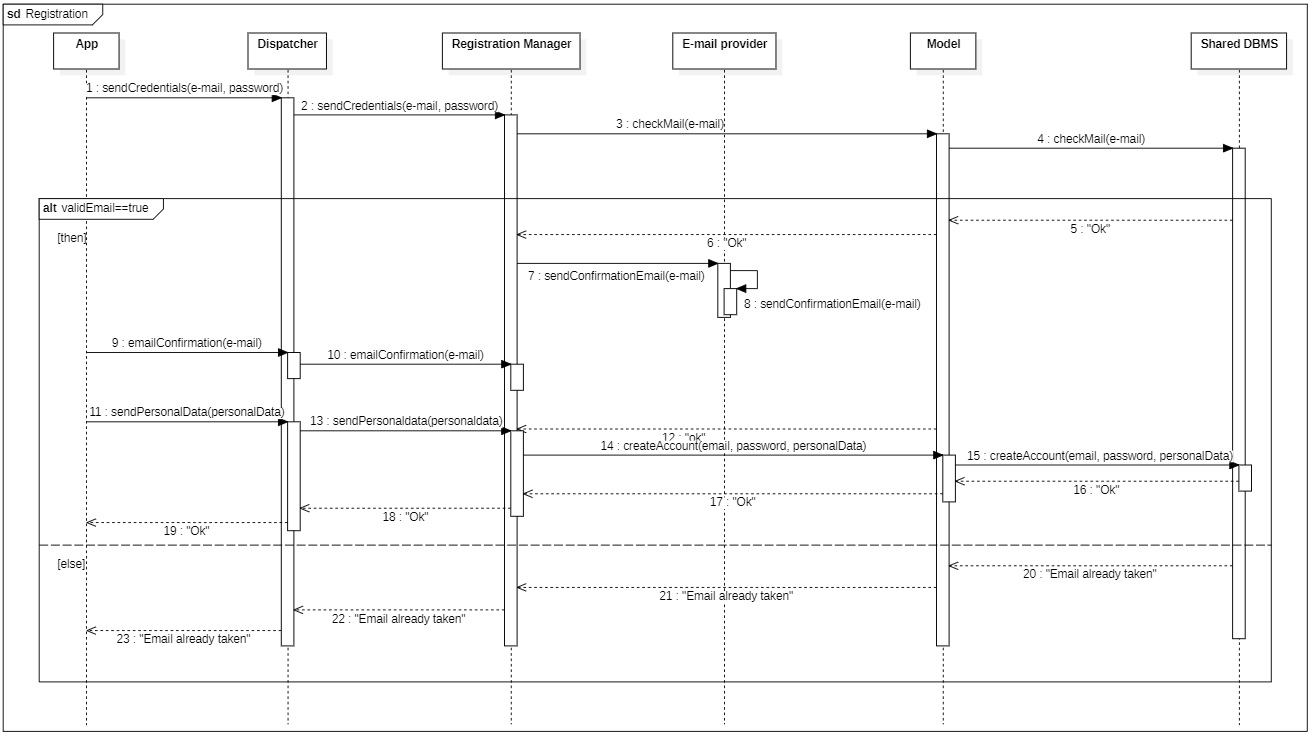
\includegraphics[width=\linewidth]{UC1.png}
\end{figure}
\noindent
This sequence diagram describes the process of a User registering in the system.\\
A registration request, containing the e-mail and password of the new user, is sent to the Dispatcher, which forwards it to the Registration Manager; the credentials are checked from it through the model, which contacts the DBMS to see if the mail is already associated to an existing account: if yes, the message is forwarded back to the app and the procedure ends.\\
If the e-mail address is available the Registration Manager sends it, through the e-mail provider of the system, the confirmation e-mail.\\
When the confirmation is done by the user, the app sends a request to the Dispatcher which notifies the Registration Manager, which is eventually able to receive the personal data of the user: when they have been inserted it sends them to the DBMS through the model and the new account is successfully created and saved into the system, then a confirmation message is sent back to the app.\\

\begin{figure}[H]
    \centering
    \textbf{[UC2] Login} \\
    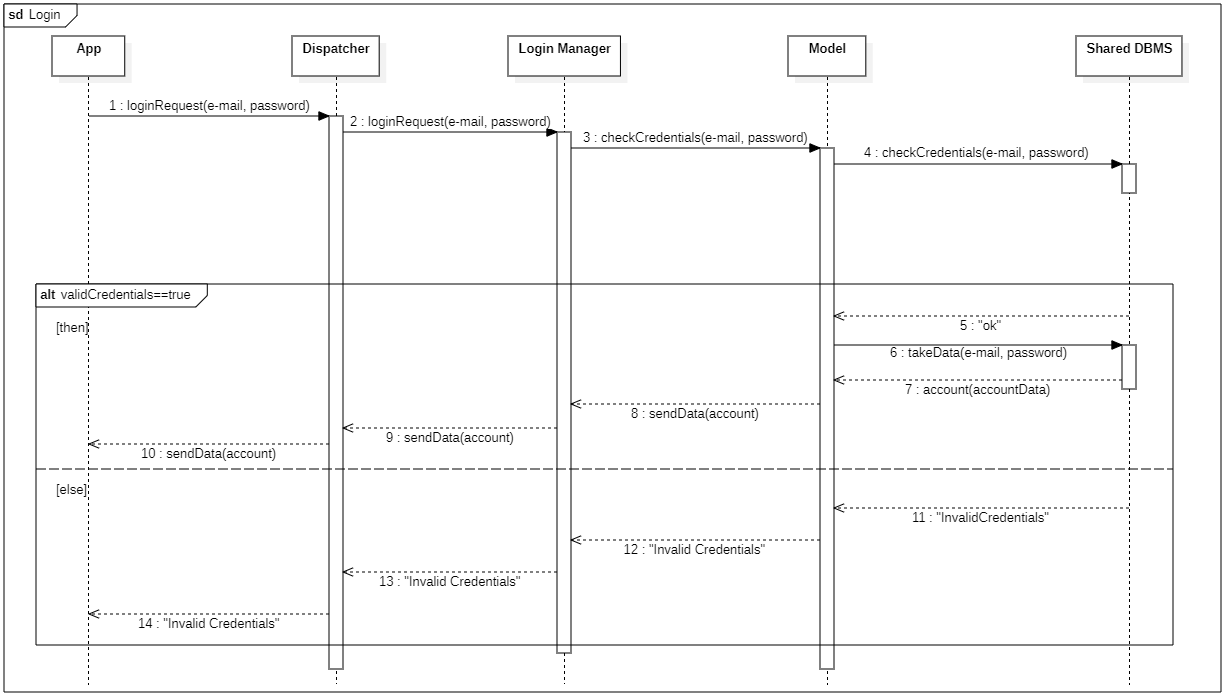
\includegraphics[width=\linewidth]{UC2.png}
\end{figure}
\noindent
This sequence diagram represents the login process of a user of the system.\\
When the App sends a Login Request, with its associated credentials to the Dispatcher, the Login Manager is contacted to check if they are effectively associated with an existing account: this is done through the Model, which can contact the DBMS and send it the credentials to be checked.\\
If the account exists, the DBMS returns its data that are forwarded back to the app, else an "Invalid Credentials" message is sent back by the database: in both cases, the procedure then ends.

\begin{figure}[H]
    \centering
    \textbf{[UC3] Create Tournament} \\
    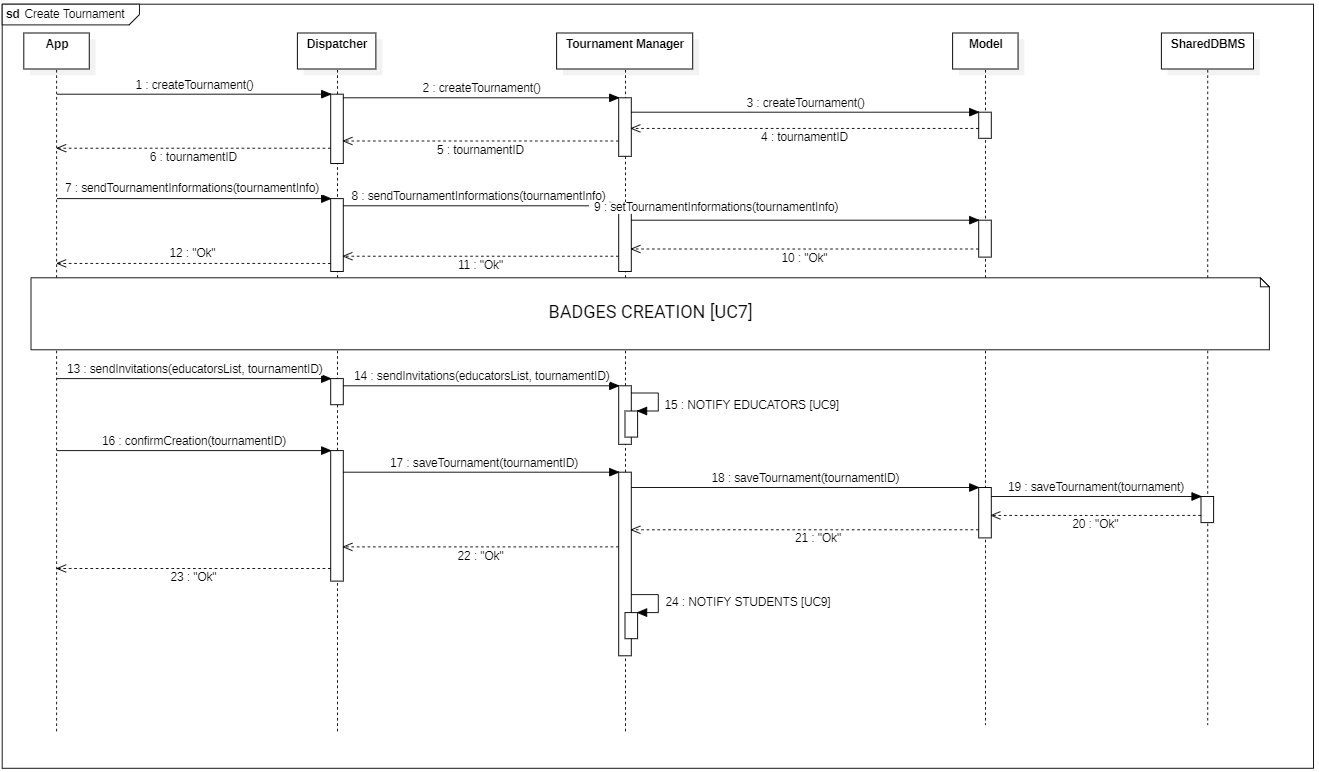
\includegraphics[width=\linewidth]{UC3.png}
\end{figure}
\noindent
This sequence diagram represents the process of creation of a Tournament by an Educator of the system.
When the process begins, a request is sent to the Dispatcher, which forwards it to the Tournament Manager: at this point, the tournament is provisionally created and is assigned a unique ID for identification.\\
When creating the Tournament, the Educator has to follow a list of steps: the first is submitting all the information and settings of the tournament, which are forwarded to the dispatcher and then saved through the Tournament Manager and the Model, but not yet in the DBMS.\\
The second step is the gamification badge creation, which will be described in detail in $[UC7]$.\\
The third is the selection of collaborators, to which the Dispatcher sends invitations through the Notification Manager: the invitations to collaborate in a tournament can be accepted by the educator at every moment.\\
After completing these steps the app sends a confirmation request to the Dispatcher which starts, contacting the Tournament manager, and finalizing the creation of the tournament, the data of which are eventually stored in the DBMS; after that, the process ends, and all the users are notified about the new created tournament.

\begin{figure}[H]
    \centering
    \textbf{[UC4] Create Battle } \\ 
    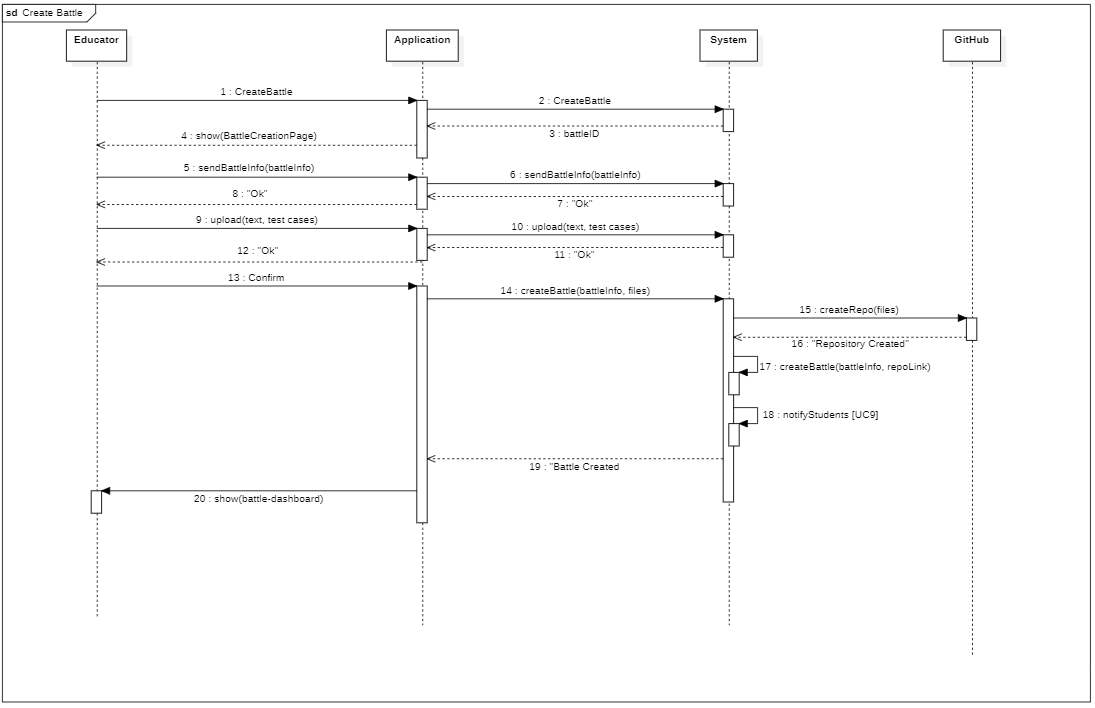
\includegraphics[width=\linewidth]{UC4.png}
\end{figure}
\noindent
This sequence diagram describes the process of battle creation by an Educator: when the process begins, a request is sent to the Dispatcher, which forwards it to the Tournament Manager: at this point, the tournament is provisionally created through the Battle Manager and is assigned a unique ID for identification.\\
The client then sends to the Dispatcher one by one all the information and settings of the battle, and the files of the exercise, including the text and test cases, that are saved to be uploaded on GitHub when the process is being finalized.\\
After that the client has to confirm the creation of the battle: when they do it the confirmation request is forwarded from the Dispatcher to the Tournament Manager, which forwards it to the right tournament's Battle Manager's instance, which provides the creation of the GitHub repository containing the files previously uploaded by the client and to store the battle's data in the DBMS through the Model, including the repository's link returned by GitHub to the Battle Manager.\\
After that, all the participants of the tournament are notified about the newly created battle and the process ends.\\

\begin{figure}[H]
    \centering
    \textbf{[UC5] Join Battle} \\
    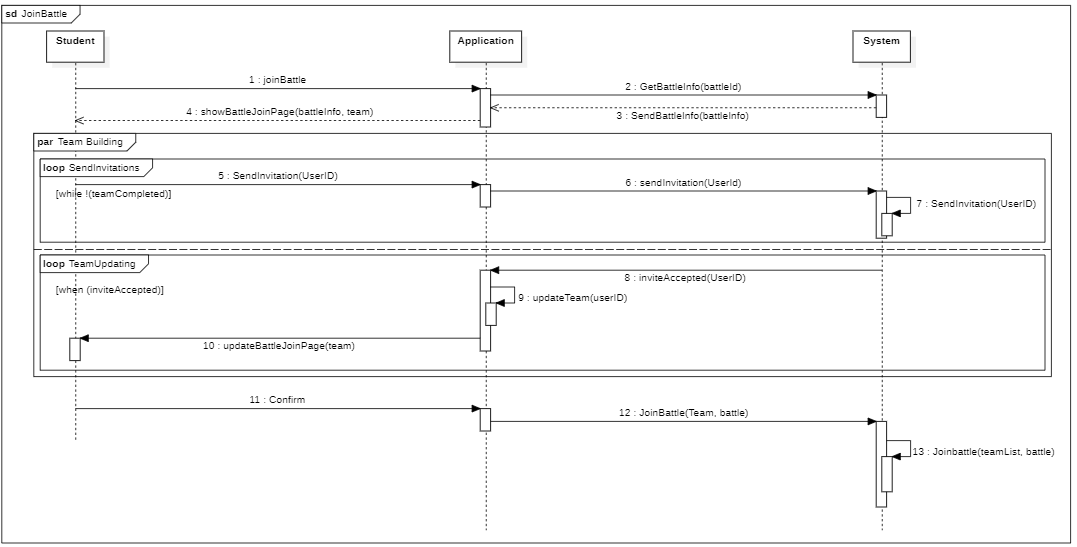
\includegraphics[width=\linewidth]{UC5.png}
\end{figure}
\noindent
This sequence diagram describes the process of joining a battle by a Student subscribed to the tournament that hosts the battle.\\
Each student can send invitations to all the other participants of the tournament to form a team: the invitations are sent through the Notification system, which is described in more detail in $[UC9]$, contacted by the Dispatcher that sends the IDs of the receiver and the tournament and battle which the invitation is referring to.\\
When the team is formed the client confirms his subscription to the Dispatcher with a specific request: the confirmation is forwarded to the Tournament manager and then to the right Battle Manager, which confirms the subscription by storing the user's team's data in the DBMS through the model.

\begin{figure}[H]
    \centering
    \textbf{[UC6] Join The Tournament} \\
    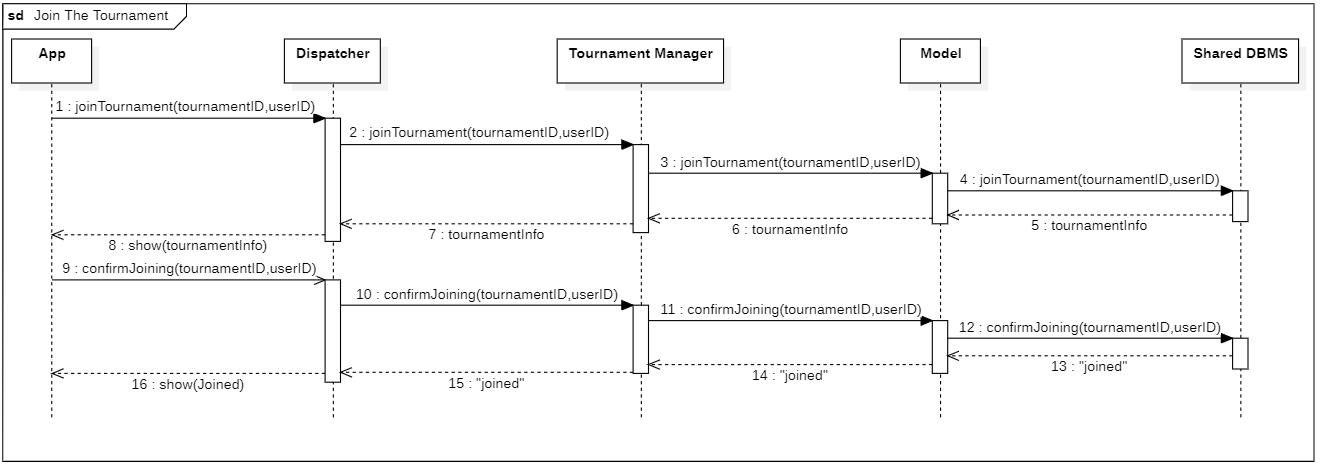
\includegraphics[width=\linewidth]{UC6.png}
\end{figure}
\noindent
This sequence diagram outlines the procedure for joining a tournament. Initially, the user sends a request to the Tournament Manager expressing the intent to join the tournament. Subsequently, the Tournament Manager retrieves information about the tournament from the Shared DBMS and provides it to the user. After reviewing the information, if the user decides to proceed with joining, they confirm the action. The Tournament Manager then updates the tournament in the DBMS to reflect the user's participation.

\begin{figure}[H]
    \centering
    \textbf{[UC7] Badge Creation} \\
    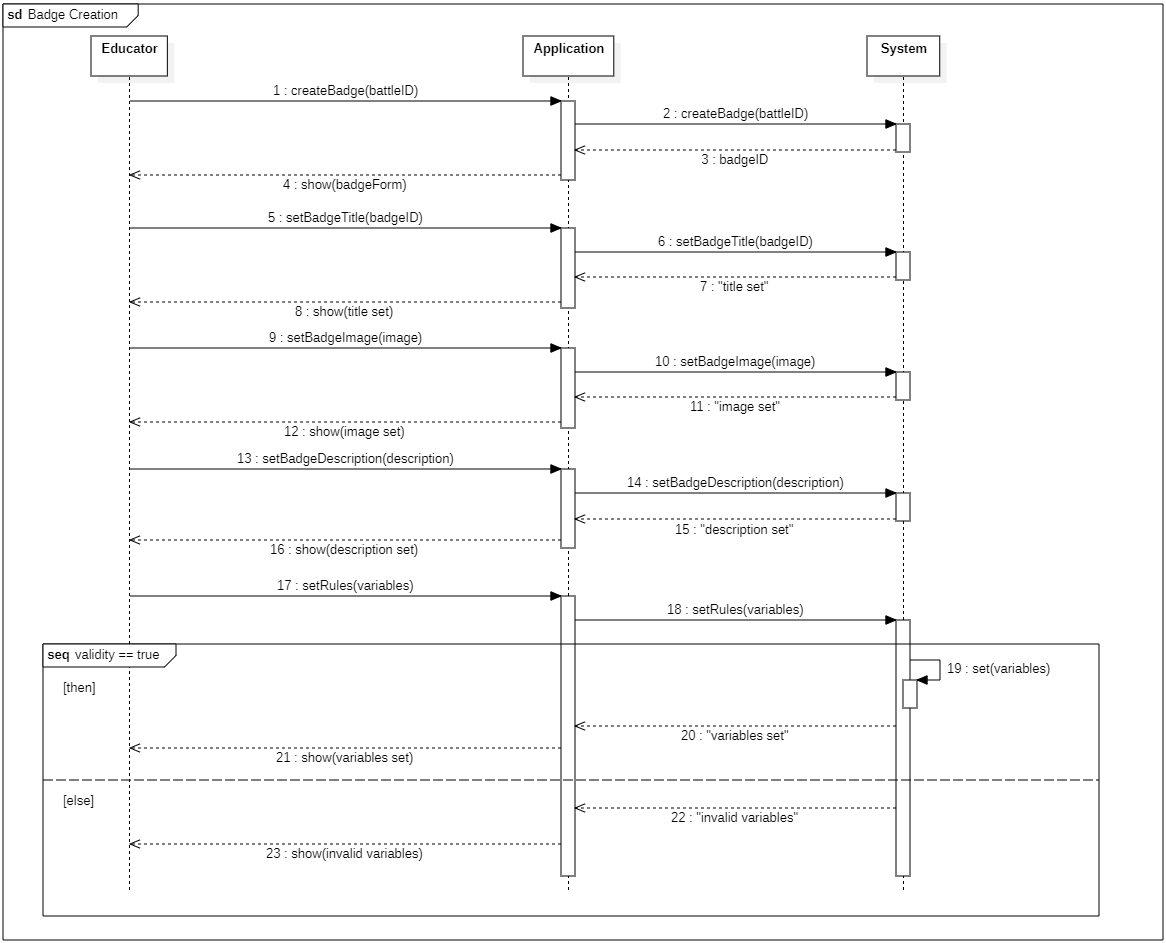
\includegraphics[width=\linewidth]{UC7.png}
\end{figure}
\noindent
This sequence diagram illustrates the process of creating a badge. To initiate the procedure, the educator sends a request to the Tournament Manager, which, through the Badge Manager, creates a new empty badge within the specified tournament and saves it in the Shared DBMS. Subsequently, a form is dispatched to the educator, who then proceeds to populate it with all the necessary information, including the rules for the badge. \\
Following this, a validation procedure ensures the rules' accuracy, and if everything checks out, the badge creation is deemed complete.

\begin{figure}[H]
    \centering
    \textbf{[UC8] Assigning a Badge} \\
    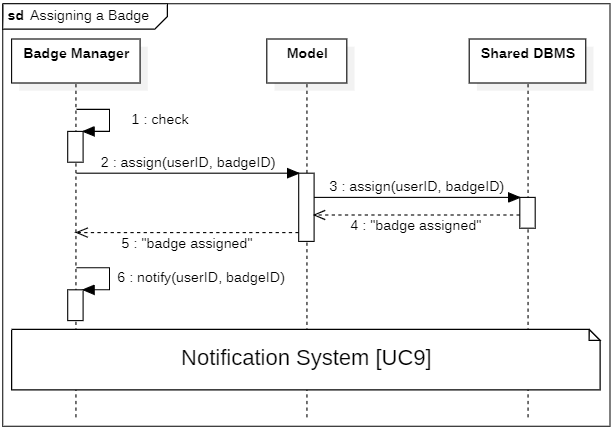
\includegraphics[width=\linewidth]{UC8.png}
\end{figure}
\noindent
This sequence diagram illustrates the process of assigning a badge. Following the conclusion of a tournament or a battle, the Badge Manager checks whether a student has fulfilled all the necessary tasks to earn a specific badge. If the criteria are met, the Badge Manager proceeds to assign the badge to the user by saving the information in the Shared DBMS. Following this, a notification is sent to the user who earned the badge, as per the notification procedure described in UC9.

\begin{figure}[H]
    \centering
    \textbf{[UC9] Notification System} \\
    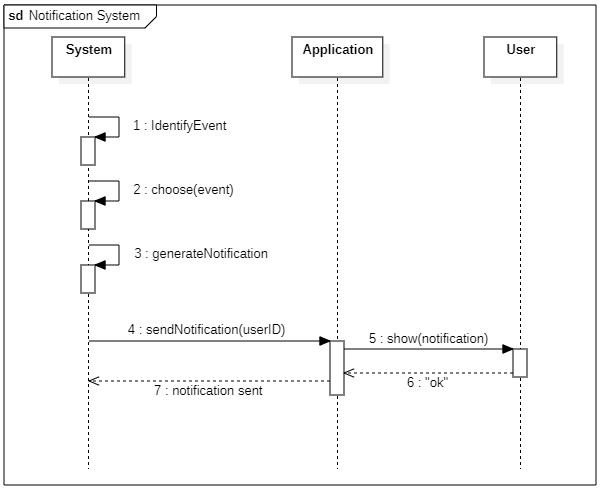
\includegraphics[width=\linewidth]{UC9.png}
\end{figure}
\noindent
This sequence diagram delineates the process of sending a notification. Upon the occurrence of a specific event, such as sending a join request or earning a badge, the Tournament Manager initiates the notification process by communicating all the notification info to the Notification Manager. Subsequently, the Notification Manager generates the notification, saves it in the Shared DBMS, and then forwards it to the App.

\begin{figure}[H]
    \centering
    \textbf{[UC10] Automated Evaluation} \\
    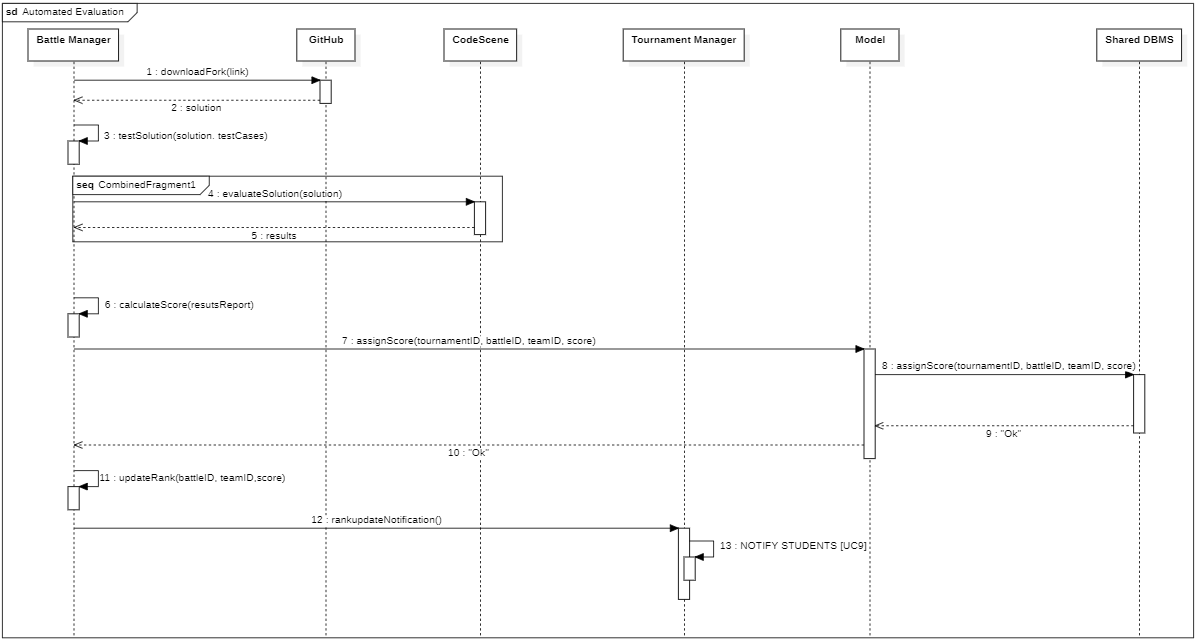
\includegraphics[width=\linewidth]{UC10.png}
\end{figure}
\noindent
This sequence diagram represents the process of automatically evaluating a solution submitted by a student for a battle.
The battle manager provides to download the solution of the student from his fork and the test cases from the battle repository on GitHub.\\
Then it executes the tests on the submitted solution and, if they are passed, proceeds to forward the files to CodeScene to be evaluated, and then, based on its results, Battle Manager computes the effective score for the solution.\\
The score is finally assigned to the Team (if the tests are not passed the score assigned in this phase will be 0), and the rank is updated: all the students of the battle are notified about the update and the procedure ends.

\begin{figure}[H]
    \centering
    \textbf{[UC11] Manual Evaluation} \\
    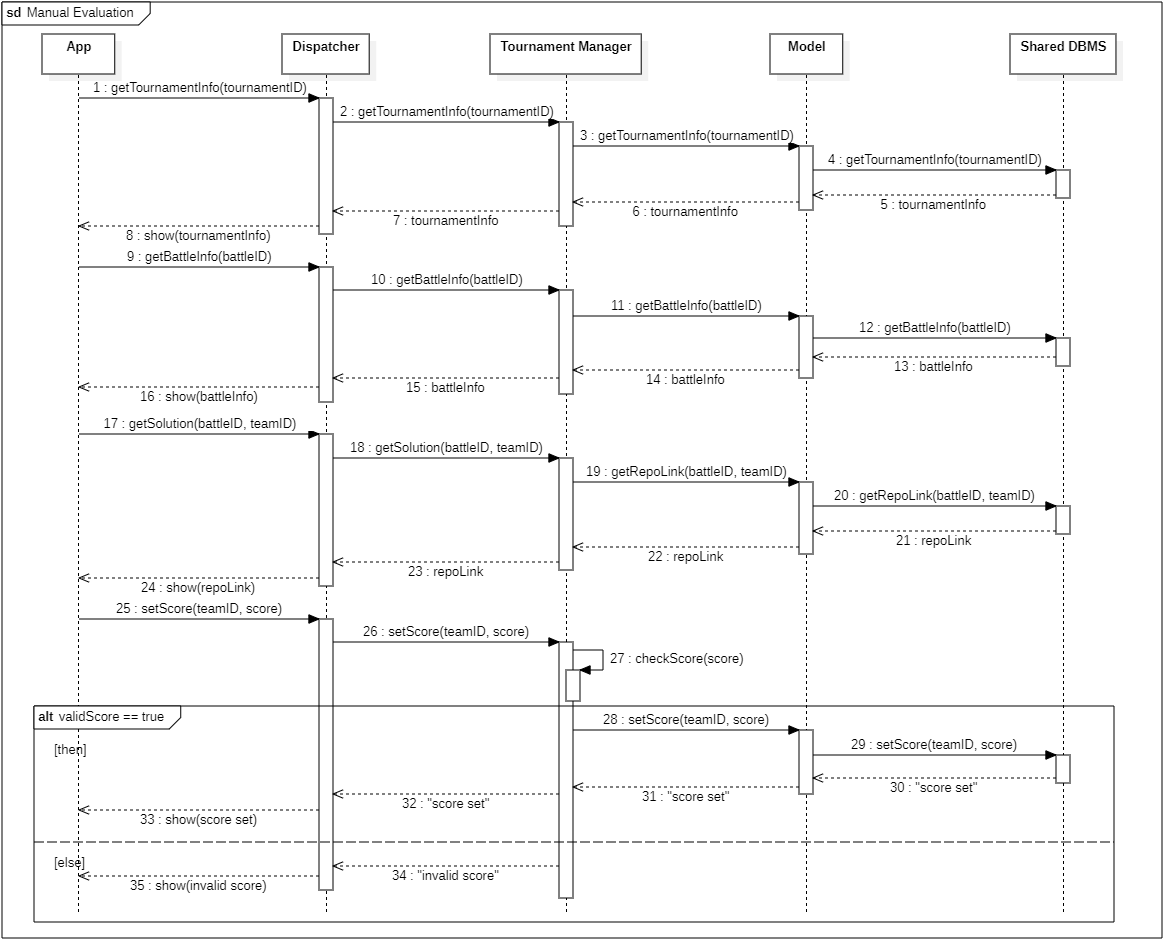
\includegraphics[width=\linewidth]{UC11.png}
\end{figure}
\noindent
This sequence diagram depicts the manual evaluation process conducted by an educator. The app initiates the procedure by sending the dispatcher a request to obtain information about a specific tournament. This request is then forwarded to the Tournament Manager, and subsequently to the Model and the Shared DBMS. \\
Once the tournament information has been retrieved, a new request is sent to the Shared DBMS to retrieve information about a specific battle within the tournament. Following this, another request is made to obtain the solution of a specific team within the battle. \\
The educator assesses the solution and assigns a score, which the Tournament Manager then verifies. If the score is deemed valid, the Tournament Manager proceeds to set the score for the solution in the Shared DBMS. Otherwise, it returns an error message to the app. \\


\begin{figure}[H]
    \centering
    \textbf{[UC12] Fork Creation} \\
    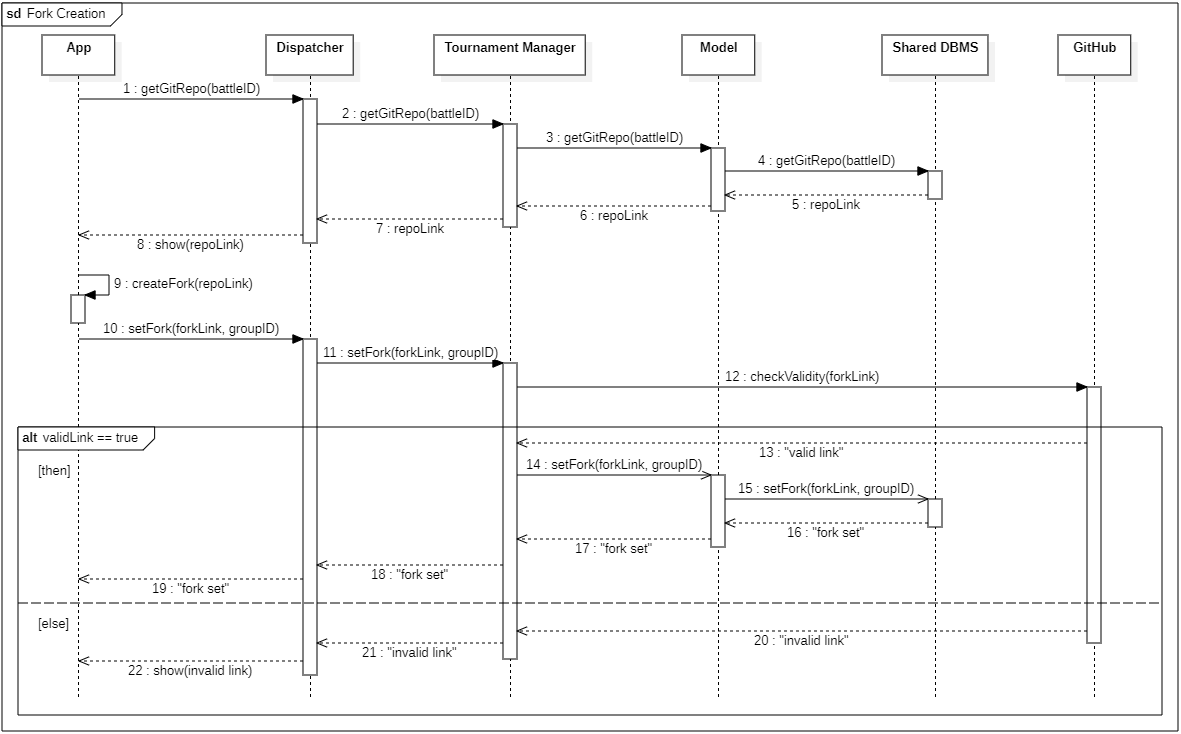
\includegraphics[width=\linewidth]{UC12.png}
\end{figure}
\noindent
This sequence diagram illustrates the fork creation process carried out by a student. The procedure commences with the app sending a request to obtain the repository link containing the problem for a specific battle. The Tournament Manager then retrieves this link from the Shared DBMS. \\
Subsequently, the student creates a new fork by accessing the GitHub repository through the provided link. The student then submits the link of the new fork to the system for processing. The Tournament Manager, in turn, interacts with the GitHub API to validate the link provided by the student. If the link is valid, the Tournament Manager saves it in the Shared DBMS and sends a confirmation message to the user. However, if the link is invalid, the system sends an error message to the user.

\begin{figure}[H]
    \centering
    \textbf{[UC13] Close Tournament} \\
    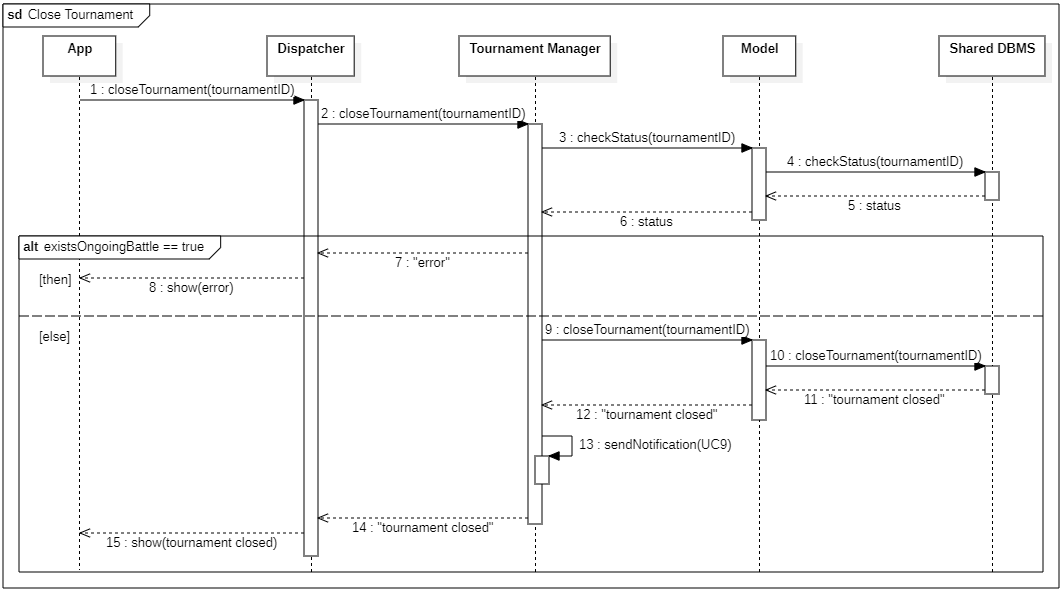
\includegraphics[width=\linewidth]{UC13.png}
\end{figure}
\noindent
This sequence diagram represents the procedure for closing a tournament, executed by the educator who created it. Initially, the app sends a request to close the tournament to the Tournament Manager, which then verifies the tournament's state through the Shared DBMS. If there are no ongoing battles within the tournament, the Tournament Manager updates the tournament state to 'closed' in the Shared DBMS and notifies all students who joined that tournament via the Notification Manager. However, if there are ongoing battles, an error message is sent to the app.

\begin{figure}[H]
    \centering
    \textbf{[UC14] Visit Profile} \\
    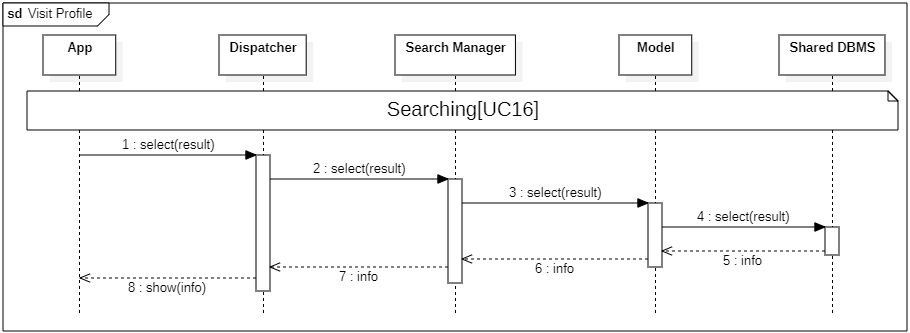
\includegraphics[width=\linewidth]{UC14.png}
\end{figure}
\noindent
This sequence diagram illustrates the process of visiting a user profile. It begins with the app initiating a request to retrieve information about a specific keyword, as described in \textbf{[UC16]}. Following the retrieval of suggested results, the app sends the selected topic to the Search Manager for information retrieval. The Search Manager then collects the information by querying the Shared DBMS. Finally, all the gathered information is sent back to the Search Manager and subsequently to the app.

\begin{figure}[H]
    \centering
    \textbf{[UC15] Joining Invitation} \\
    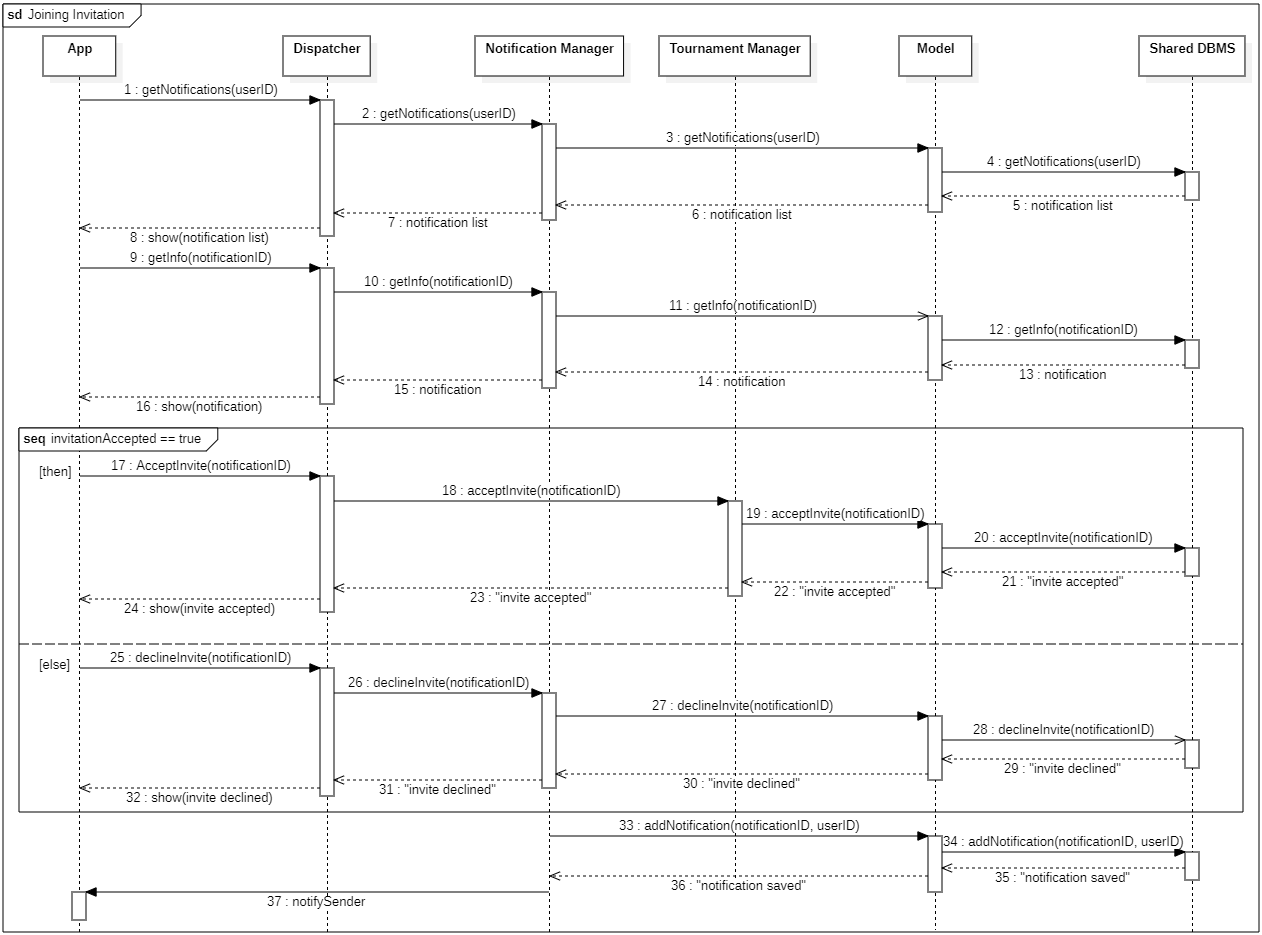
\includegraphics[width=\linewidth]{UC15.png}
\end{figure}
\noindent
This sequence diagram outlines the process of a user joining an invitation. Initially, the app sends a request to the Notification Manager to retrieve all active notifications from the Shared DBMS. Subsequently, the app requests information about a specific notification from the Notification Manager, which obtains the information by accessing the Shared DBMS. \\
If the user chooses to accept the invitation, the app sends a request to the Tournament Manager, which adds the user to the invited group. In the case of declining the invitation, the app sends a request to the Notification Manager, which handles the decline process. After the invitation is either accepted or declined, the Notification Manager creates a new notification, saves it in the Shared DBMS, and then sends the new notification to all designated users.

\begin{figure}[H]
    \centering
    \textbf{[UC16] Searching} \\
    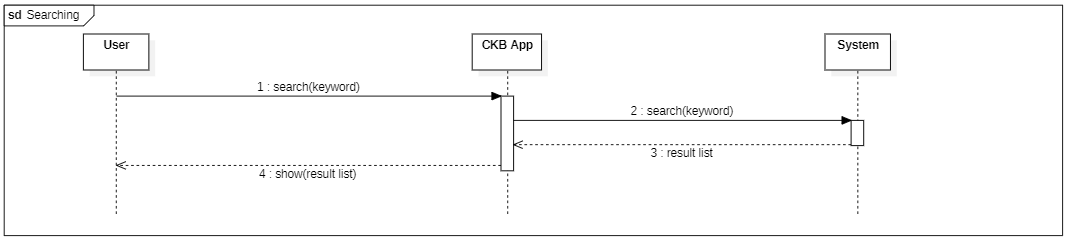
\includegraphics[width=\linewidth]{UC16.png}
\end{figure}
\noindent
This sequence diagram illustrates the user's search procedure involving the insertion of a specific keyword. The app sends a request to the Search Manager, which queries the Shared DBMS to retrieve a list of results for the specified keyword. The Search Manager then sends this list to the app.

\subsection{Component interfaces}
This section outlines the methods that each component interface extends to other components.
\begin{itemize}
    \item \textbf{Dispatcher}
        \begin{itemize}
            \item loginRequest(e-mail, password)
            \item sendCredentials(e-mail, password)
            \item emailConfirmation(e-mail)
            \item sendPersonalData(personalData)
            \item createTournament()
            \item sendTournamentInformations(tournamentInfo)
            \item sendInvitations(educatorsList, tournamentID)
            \item confirmCreation(tournamentID)
            \item createBattle(tournamentID, battleInfo)
            \item setBattleInfo(tournamentID, battleId, battleInfo)
            \item uploadFiles(tournamentID, battleID, text, testCases)
            \item saveBattle(tournamentID, battleID)
            \item getBattleInfo(tournamentID, battleID)
            \item joinBattle(tournamentID, battleID, userID)
            \item sendInvitation(UserID, TournamentID, battleID)
            \item joinBattle(teamID, tournamentID, battleID)
            \item joinTournament(tournamentID, userID)
            \item confirmJoining(tournamentID, userID)
            \item createBadge(battleID)
            \item setBadgeTitle(badgeID, title)
            \item setBadgeImage(badgeID, image)
            \item setBadgeDescription(badgeID, description)
            \item setRules(badgeID, variables)
            \item getTournamentInfo(tournamentID)
            \item getBattleInfo(battleID)
            \item getSolution(battleID, teamID)
            \item setScore(teamID, score)
            \item getGitRepo(battleID)
            \item setFork(forkLink, groupID)
            \item closeTournament(tournamentID)
            \item select(result)
            \item getNotifications(userID)
            \item getInfo(notificationID)
            \item acceptInvite(notificationID)
            \item declineInvite(notificationID)
            \item search(keyword)
        \end{itemize}
    \item\textbf{Registration Manager}
        \begin{itemize}
            \item sendCredentials(e-mail, password)
            \item emailConfirmation(e-mail)
            \item sendPersonalData(personalData)
        \end{itemize}
     \item\textbf{Login Manager}
        \begin{itemize}
            \item loginRequest(e-mail, password)
        \end{itemize}
    \item \textbf{Tournament Manager}
        \begin{itemize}
            \item createTournament()
            \item sendTournamentInformations(tournamentInfo)
            \item saveTournament(tournamentID)
            \item createBattle(tournamentID)
            \item setBattleInfo(tournamentID, battleID, battleInfo)
            \item uploadFiles(tournamentID, battleID, text, testCases)
            \item saveBattle(tournamentID, battleID)
            \item getBattleInfo(tournamentID, battleID)
            \item joinBattle(tournamentID, battleID, userID)
            \item joinBattle(teamID, tournamentID, battleID)
            \item joinTournament(tournamentID,userID)
            \item confirmJoining(tournamentID,userID)
            \item createBadge(battleID)
            \item setBadgeTitle(badgeID, title)
            \item setBadgeImage(badgeID, image)
            \item setBadgeDescription(badgeID, description)
            \item setRules(badgeID, variables)
            \item getTournamentInfo(tournamentID)
            \item getSolution(battleID, teamID)
            \item setScore(teamID, score)
            \item getGitRepo(battleID)
            \item setFork(forkLink, groupID)
            \item closeTournament(tournamentID)
            \item acceptInvite(notificationID)
        \end{itemize}
    \item \textbf{Model}
        \begin{itemize}
            \item checkMail(e-mail)
            \item createAccount(e-mail, password, personalData)
            \item checkCredentials(e-mail, password)
            \item createTournament()
            \item setTournamentInformations(tournamentInfo)
            \item saveTournament(tournamentID)
            \item createBattle()
            \item setBattleInfo(battleInfo)
            \item setFiles(battleID, text, testCases)
            \item saveBattle(battle)
            \item getBattleInfo(tournamentID, battleID)
            \item createTeam(userID, battleID)
            \item joinBattle(teamID, tournamentID, battleID)
            \item joinTournament(tournamentID,userID)
            \item confirmJoining(tournamentID,userID)
            \item createBadge(battleID)
            \item setBadgeTitle(badgeID, title)
            \item setBadgeImage(badgeID, image)
            \item setBadgeDescription(badgeID, description)
            \item setRules(variables)
            \item assign(userID, badgeID)
            \item sendNotification(userID, notificationID)
            \item addNotification(notificationID, userID)
            \item getTournamentInfo(tournamentID)
            \item getBattleInfo(battleID)
            \item getRepoLink(battleID, teamID)
            \item setScore(teamID, score)
            \item getGitRepo(battleID)
            \item setFork(forkLink, groupID)
            \item checkStatus(tournamentID)
            \item closeTournament(tournamentID)
            \item select(result)
            \item getNotifications(userID)
            \item getInfo(notificationID)
            \item acceptInvite(notificationID)
            \item declineInvite(notificationID)
            \item search(keyword)
        \end{itemize}
    \item \textbf{Notification Manager}
        \begin{itemize}
            \item sendInvitation(educatorsList, tournamentID)
            \item sendInvitation(UserID, TournamentID, battleID)
            \item sendNotification(info)
            \item getNotifications(userID)
            \item getInfo(notificationID)
            \item declineInvite(notificationID)
        \end{itemize}
    \item \textbf{Search Manager}
        \begin{itemize}
            \item select(result)
            \item search(keyword)
        \end{itemize}
    \item \textbf{Shared DBMS}
        \begin{itemize}
            \item checkMail(e-mail)
            \item createAccount(e-mail, password, personalData)
            \item checkCredentials(e-mail, password)  
            \item takeData(e-mail, password)
            \item saveTournament(tournament)
            \item saveBattle(battle)
            \item getBattleInfo(tournamentID, battleID)
            \item joinBattle(teamID, tournamentID, battleID)
            \item joinTournament(tournamentID,userID)
            \item confirmJoining(tournamentID,userID)
            \item createBadge(battleID)
            \item setBadgeTitle(badgeID, title)
            \item setBadgeImage(badgeID, image)
            \item setBadgeDescription(badgeID, description)
            \item setRules(variables)
            \item assign(userID, badgeID)
            \item addNotification(notificationID, userID)
            \item getTournamentInfo(tournamentID)
            \item getRepoLink(battleID, teamID)
            \item setScore(teamID, score)
            \item getGitRepo(battleID)
            \item setFork(forkLink, groupID)
            \item checkStatus(tournamentID)
            \item closeTournament(tournamentID)
            \item select(result)
            \item getNotifications(userID)
            \item getInfo(notificationID)
            \item acceptInvite(notificationID)
            \item declineInvite(notificationID)
            \item search(keyword)
        \end{itemize}
\end{itemize}
\newpage
\subsection{Selected architectural styles and patterns}
\subsubsection{3-tier Architecture}
CKB will be built upon a 3-tier architecture, providing numerous benefits through the modularization of the system into three independent layers or tiers:
\begin{itemize}
    \item \textbf{Presentation Tier:} This top-level tier encompasses the customer interface, focusing on rearranging data received from the application tier to present it in a more intuitive and comprehensible manner to customers.
    \item \textbf{Application Tier:} This tier houses the logic of the application, governing decision-making and calculations. It plays a crucial role in passing and processing data between the surrounding layers.
    \item \textbf{Data Tier:} This tier incorporates the Database system and offers an API to the application tier for accessing and managing data stored in the database.
\end{itemize}
Adopting this architecture ensures heightened flexibility by allowing the development and updating of specific parts of the system independently. Additionally, the middle tier between the client and data server enhances data security, as information is accessed through the application layer rather than directly by the client.

\subsubsection{Model View Controller}
The Model-View-Controller pattern is used for the system implementation on both web and smartphone app, it consists in three main components:
\begin{itemize}
    \item \textbf{Model:} Houses the application's data and offers methods for its manipulation.
    \item \textbf{View:} Encompasses various visual representations of the data.
    \item \textbf{Controller:} Intermediary between the model and the view. Upon event occurrences, it executes predefined reactions, which may involve operations on the model, reflecting changes on the view.
\end{itemize}
The division of responsibilities among these three elements fosters a heightened degree of decoupling among components. This architectural choice brings forth a multitude of advantages, including improved reusability and a simplified implementation process, among other benefits.

\subsubsection{Observer}
Within the code kata application's architecture, the Observer Pattern intricately manages the notification system and invitation mechanism. This design choice allows components responsible for sending invitations to dynamically notify and update observers, ensuring a decoupled and responsive system that adheres to a modular and scalable paradigm.

\subsubsection{Mediator}
The mediator pattern, a behavioral design pattern, serves the purpose of reducing coupling between communicating modules. Acting as an intermediary, the mediator component sits between two or more objects, shielding them from the need to delve into each other's implementation details. Within our system, multiple mediators play pivotal roles, fostering effective communication and maintaining a decoupled architecture.
\begin{itemize}
    \item \textbf{Registration Manager:} Serving as a mediator, it establishes a link between the internal components of the application server and the external email provider. This approach ensures enhanced flexibility for the system, allowing seamless adaptation to changes in the email provider by making modifications solely to the Registration Manager.
    \item \textbf{Model:} Due to the implementation of the MVC pattern, the Model undertakes the role of a mediator among its various tasks. Specifically, when data access is required, the Model acts as an intermediary between the Shared DBMS and the other components.
    \item \textbf{Battle Manager:} Serving as a mediator between the Tournament Manager and external components, namely GitHub and CodeScene, this component ensures that changes in GitHub or CodeScene APIs exclusively impact the Battle Manager, which can be modified accordingly.
    \item \textbf{Tournament Manage:} Functioning as a mediator, it connects its internal components, namely the Battle Manager and Badge Manager, with other internal components within the system.
\end{itemize}


\subsection{Other design decisions}
In this paragraph we are going to present some design decisions taken to make the system work as efficiently and reliably as possible:
\begin{itemize}
    \item \textbf{Reliability}: Firewalls have been added to the system to protect it from all possible threats from the outside which can affect its integrity or performance making it unable to work properly as it should.
    \item \textbf{Efficiency}: Load Balancers have been inserted in the system to increase its availability managing in the most efficient possible way the requests that are coming from the clients.
    The load balancers can avoid overload cases for the system resulting in possible bottlenecks that could considerably affect the system's performance in terms of response speed.
    \item \textbf{Data Storage}: The choice to store all data of the system in a single shared DBMS has been taken in consequence of their homogeneity and the interconnection between them: all data have to be used by all the users, regardless of whether they are Students or Educators, it's so not necessary to divide them, cause the economic and space cost of that choice wouldn't result in an enough considerable advantage in terms of efficiency for the system.
\end{itemize}

\section{User Interface Design}


\begin{figure}[H]
    \centering
    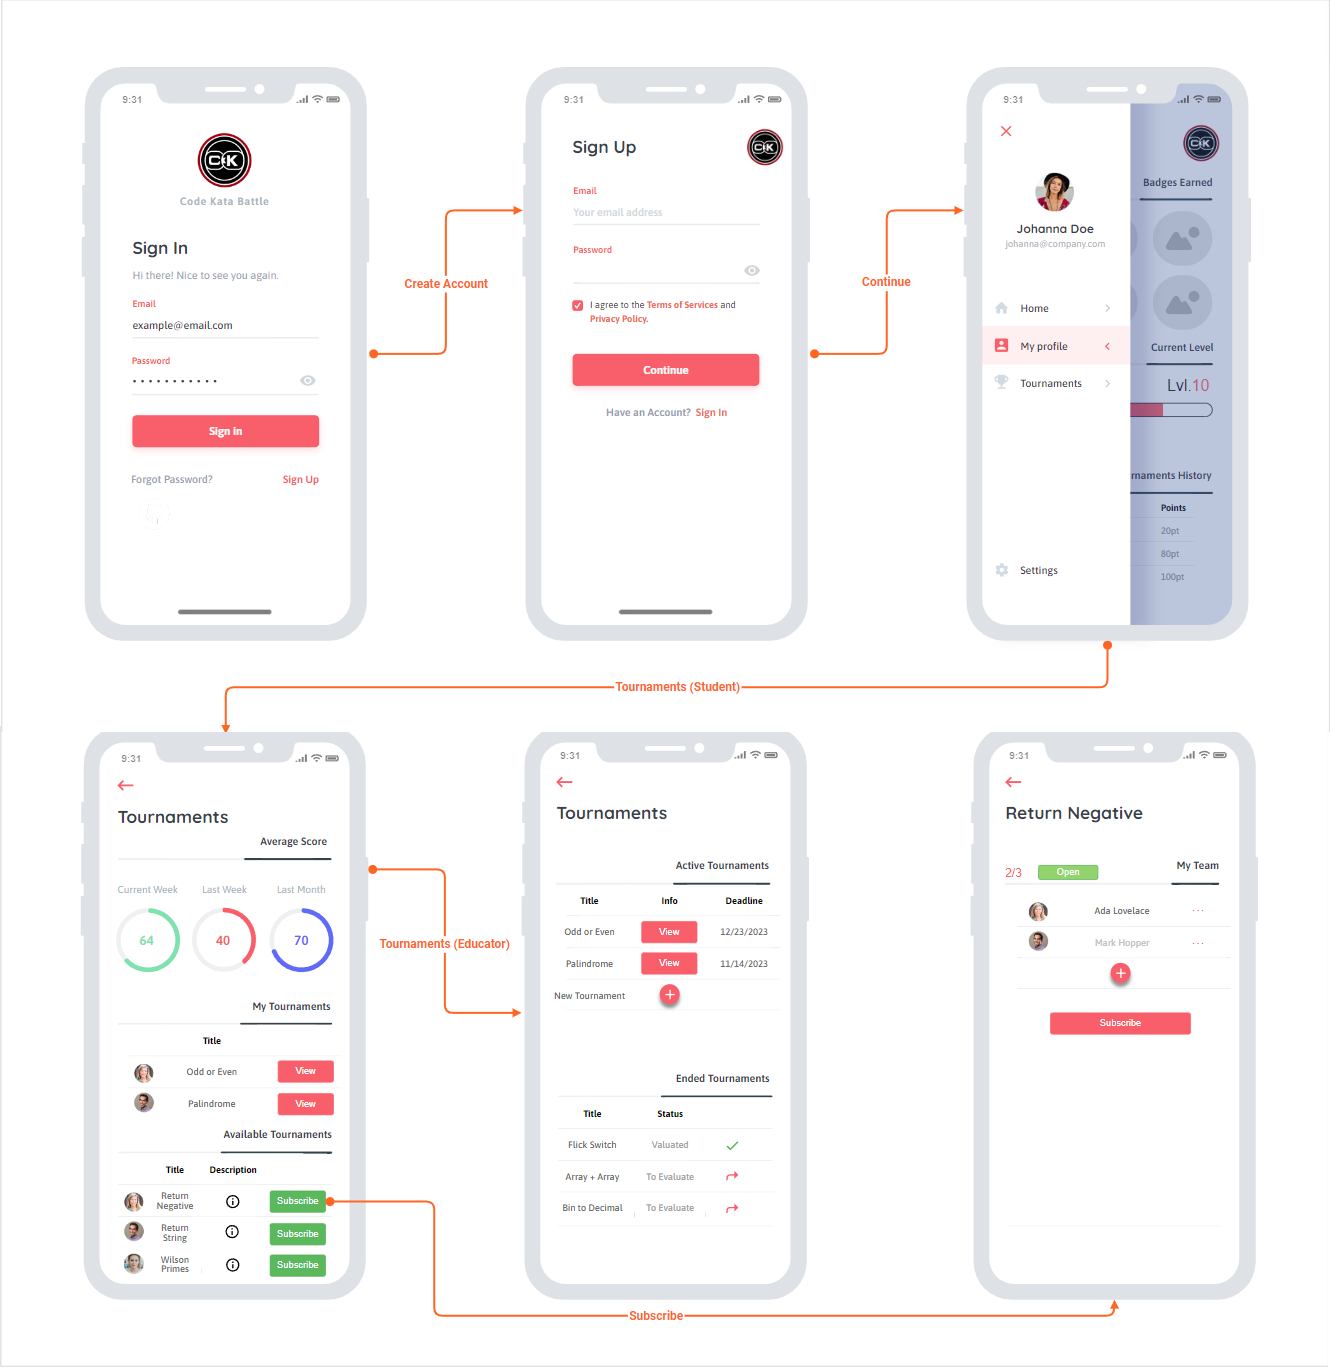
\includegraphics[width=\linewidth]{Mobile UI.png}
    \caption{General UI}
\end{figure}

\begin{figure}[H]
    \centering
    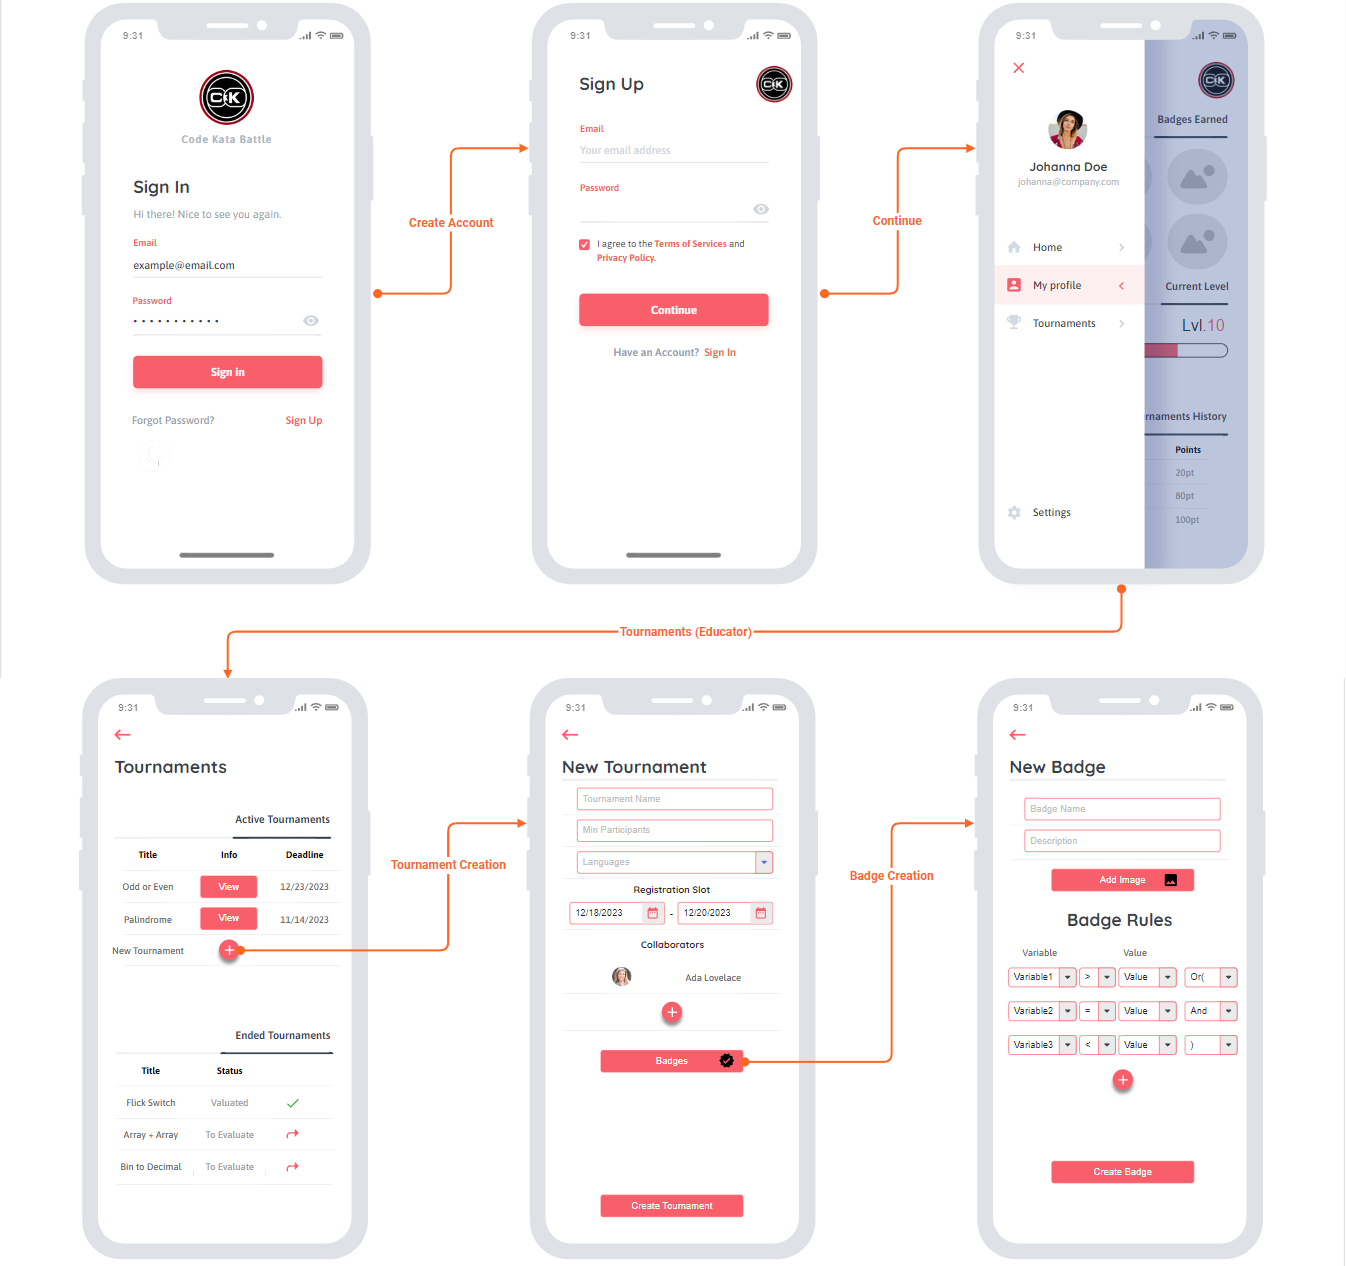
\includegraphics[width=\linewidth]{Mobile UI ED.png}
    \caption{Tournament and Badge creation}
\end{figure}

\begin{figure}[H]
    \centering
    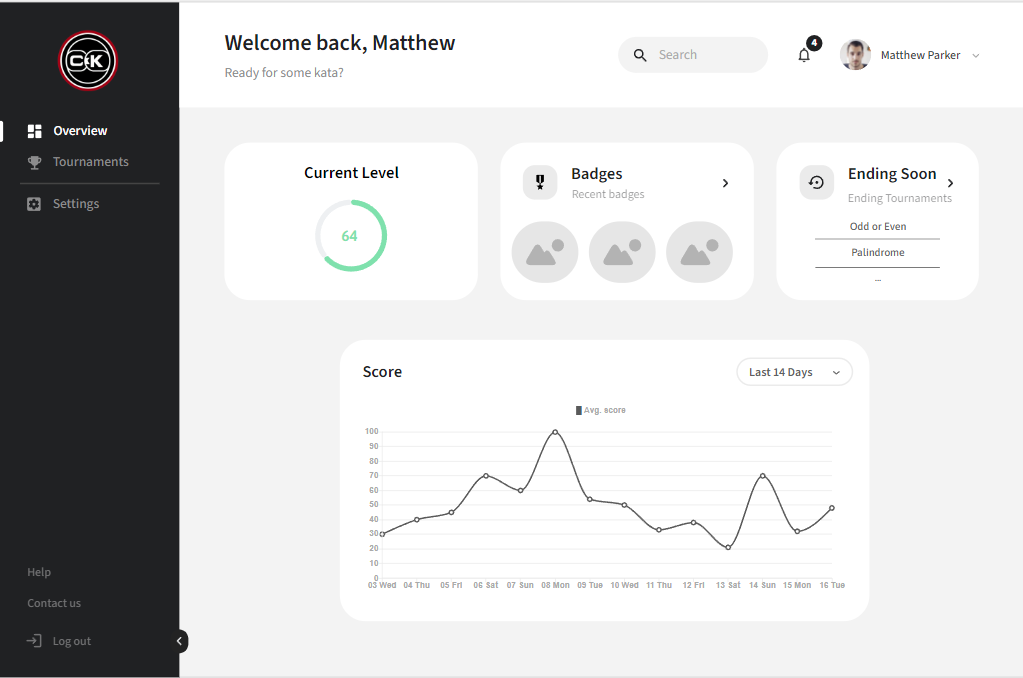
\includegraphics[width=\linewidth]{Web UI.png}
    \caption{Web UI Overview}
\end{figure}

\begin{figure}[H]
    \centering
    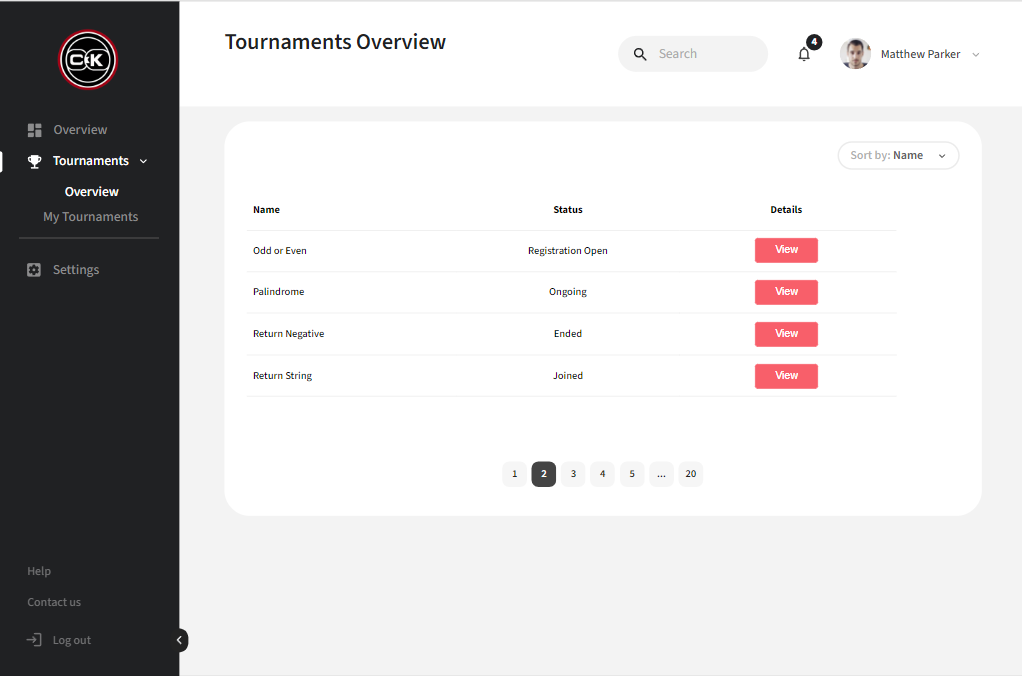
\includegraphics[width=\linewidth]{Web UI 2.png}
    \caption{Web UI Tournament Overview}
\end{figure}

\begin{figure}[H]
    \centering
    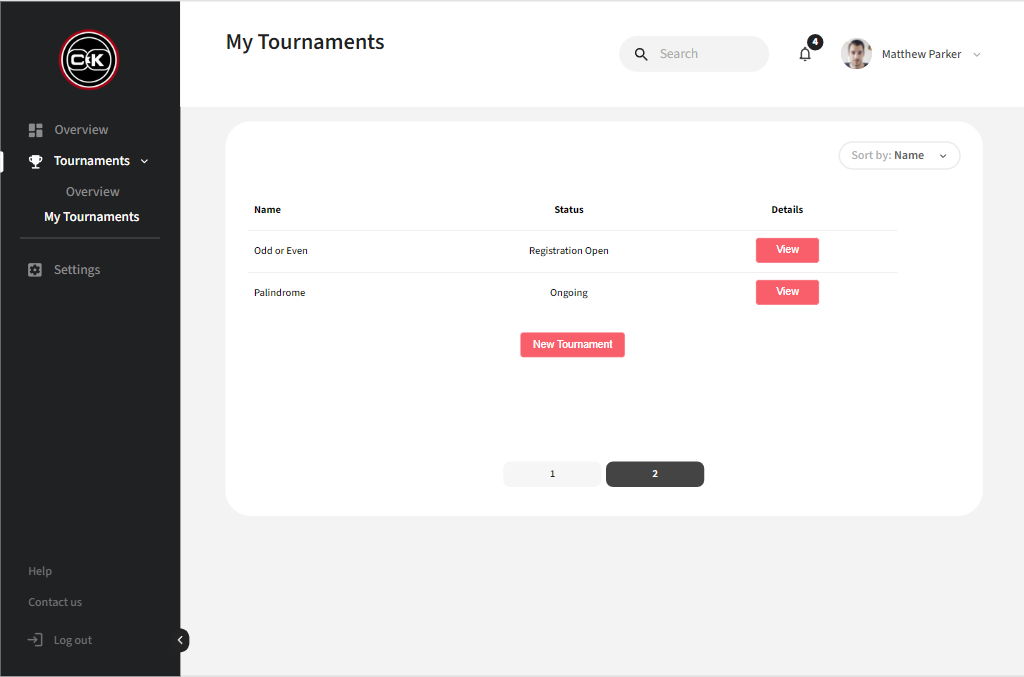
\includegraphics[width=\linewidth]{Web UI 3.png}
    \caption{Web UI My Tournament view}
\end{figure}

\begin{figure}[H]
    \centering
    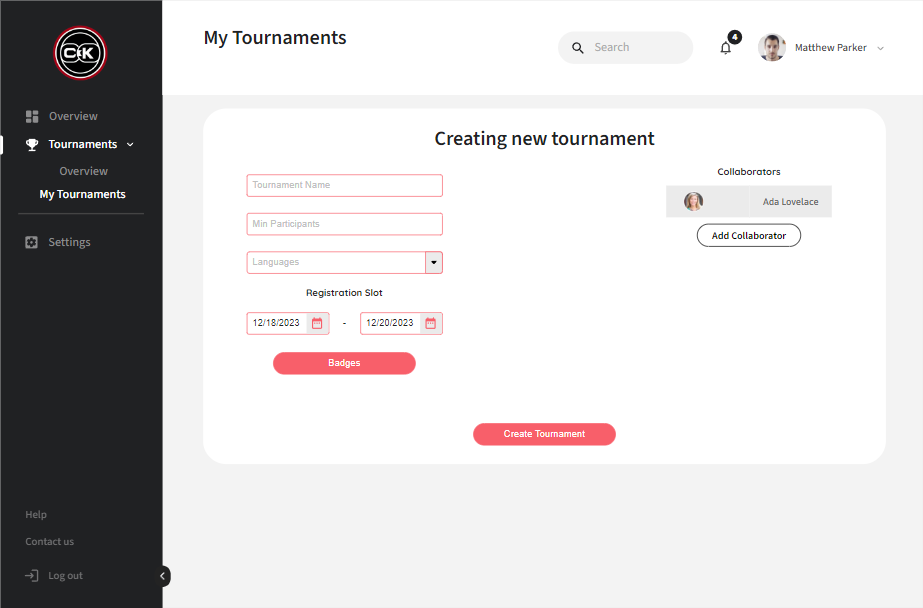
\includegraphics[width=\linewidth]{Web UI 4.png}
    \caption{Web UI Tournament creation view}
\end{figure}

\begin{figure}[H]
    \centering
    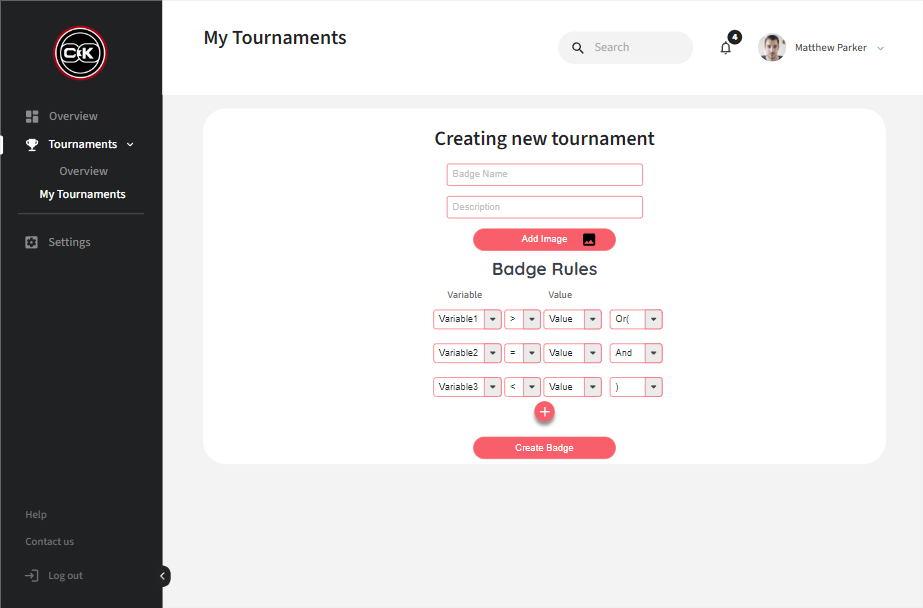
\includegraphics[width=\linewidth]{Web UI 5.png}
    \caption{Web UI Badge creation view}
\end{figure}
\newpage
\section{Requirements Traceability}
This section of the document details the design elements associated with each requirement outlined in the RASD. The following tables map these design elements to their respective requirements. \\

\begin{table}[H]
 \renewcommand{\arraystretch}{1.5}
    \centering
    \begin{tabular}{|l|p{10cm}|}
        \hline
        \textbf{Requirements} & $[FR1]$ The system allows Users to sign up \\
        \hline
        \textbf{Components} & 
        \begin{itemize}[align=left, topsep=0pt, partopsep=0pt]
            \item Smartphone App
            \item Web App
            \item Web Server
            \item Application Server:
            \begin{itemize}
                \item Dispatcher
                \item Registration Manager
                \item Model
            \end{itemize}
            \item Shared DBMS 
        \end{itemize} \\
        \hline
    \end{tabular}
\end{table}

\begin{table}[H]
 \renewcommand{\arraystretch}{1.5}
    \centering
    \begin{tabular}{|l|p{10cm}|}
        \hline
        \textbf{Requirements} & $[FR2]$ The system allows Users to log in \\
        \hline
        \textbf{Components} & 
        \begin{itemize}[align=left, topsep=0pt, partopsep=0pt]
            \item Smartphone App
            \item Web App
            \item Web Server
            \item Application Server:
            \begin{itemize}
                \item Dispatcher
                \item Login Manager
                \item Model
            \end{itemize}
            \item Shared DBMS 
        \end{itemize} \\
        \hline
    \end{tabular}
\end{table}

\begin{table}[H]
 \renewcommand{\arraystretch}{1.5}
    \centering
    \begin{tabular}{|l|p{10cm}|}
        \hline
        \textbf{Requirements} & $[FR3]$ The system allows Educators to create tournaments \\
        \hline
        \textbf{Components} & 
        \begin{itemize}[align=left, topsep=0pt, partopsep=0pt]
            \item Smartphone App
            \item Web App
            \item Web Server
            \item Application Server:
            \begin{itemize}
                \item Dispatcher
                \item Tournament Manager
                \begin{itemize}
                    \item Badge Manager
                    \item Battle Manager
                \end{itemize}
                \item Model
            \end{itemize}
            \item Shared DBMS 
        \end{itemize} \\
        \hline
    \end{tabular}
\end{table}

\begin{table}[H]
 \renewcommand{\arraystretch}{1.5}
    \centering
    \begin{tabular}{|l|p{10cm}|}
        \hline
        \textbf{Requirements} & 
        \vspace{-0.6cm}
        \begin{itemize}[label={}, left=0pt, align=left, itemsep=5pt]
            \item $[FR4]$ The system allows Educators to set a deadline for subscribing to the tournament
            \item $[FR5]$ The System allows Educators to set a list of programming languages that will be used in the tournament
            \item $[FR6]$ The system allows Educators to invite other Educators as collaborators for a tournament
            \item $[FR18]$ The system allows Students to join a tournament
            \item $[FR22]$ The system allows Educators to see the list of the active tournaments they have created
            \item $[FR23]$ The system allows Students to see the list of the active tournaments they have joined
        \end{itemize} \\
        \hline
        \textbf{Components} & 
        \begin{itemize}[align=left, topsep=0pt, partopsep=0pt]
            \item Smartphone App
            \item Web App
            \item Web Server
            \item Application Server:
            \begin{itemize}
                \item Dispatcher
                \item Tournament Manager
                \item Model
            \end{itemize}
            \item Shared DBMS 
        \end{itemize} \\
        \hline
    \end{tabular}
\end{table}

\begin{table}[H]
 \renewcommand{\arraystretch}{1.5}
    \centering
    \begin{tabular}{|l|p{10cm}|}
        \hline
        \textbf{Requirements} &
        \vspace{-0.6cm}
        \begin{itemize}[label={}, left=0pt, align=left, itemsep=5pt]
            \item $[FR7]$ The system allows Educators to set the number of battles in a tournament
            \item $[FR9]$ The system allows Educators to set a deadline for the subscription to the battle
            \item $[FR10]$ The system allows Educators to set a deadline for the submission of the solutions to the battle
            \item $[FR11]$ The System allows educators to choose which of the languages of the tournament will be used in each battle
            \item $[FR13]$ The system allows Educators to set the maximum number of students per team in a battle
            \item $[FR14]$ The system allows Educators to choose whether and when the scores will be assigned in an automatic way or also through manual verification by themselves
            \item $[FR20]$ The system allows Students to join a battle
            \item $[FR21]$ The system allows Students to know about the provisional scores of all students, updated for every solution submitted, for the duration of a battle
        \end{itemize} \\
        \hline
        \textbf{Components} & 
        \begin{itemize}[align=left, topsep=0pt, partopsep=0pt]
            \item Smartphone App
            \item Web App
            \item Web Server
            \item Application Server:
            \begin{itemize}
                \item Dispatcher
                \item Tournament Manager
                \begin{itemize}
                    \item Battle Manager
                \end{itemize}
                \item Model
            \end{itemize}
            \item Shared DBMS 
        \end{itemize} \\
        \hline
    \end{tabular}
\end{table}

\begin{table}[H]
 \renewcommand{\arraystretch}{1.5}
    \centering
    \begin{tabular}{|l|p{10cm}|}
        \hline
        \textbf{Requirements} &
        \vspace{-0.6cm}
        \begin{itemize}[label={}, left=0pt, align=left, itemsep=5pt]
            \item $[FR8]$ The system allows Educators to create battles
            \item $[FR12]$ The System allows Educators to upload the files with the text of the problem and test cases for the battle
        \end{itemize} \\
        \hline
        \textbf{Components} & 
        \begin{itemize}[align=left, topsep=0pt, partopsep=0pt]
            \item Smartphone App
            \item Web App
            \item Web Server
            \item Application Server:
            \begin{itemize}
                \item Dispatcher
                \item Tournament Manager
                \begin{itemize}
                    \item Battle Manager
                \end{itemize}
                \item Model
            \end{itemize}
            \item GitHub
            \item Shared DBMS 
        \end{itemize} \\
        \hline
    \end{tabular}
\end{table}

\begin{table}[H]
 \renewcommand{\arraystretch}{1.5}
    \centering
    \begin{tabular}{|l|p{10cm}|}
        \hline
        \textbf{Requirements} &
        \vspace{-0.6cm}
        \begin{itemize}[label={}, left=0pt, align=left, itemsep=5pt]
            \item $[FR15]$ The system allows Educators to create badges for a specific tournament
            \item $[FR16]$ The system allows Educators to build the requirements for achieving a badge
            \item $[FR17]$ The system allows Students to see what the active badges are in a tournament and what they have to do to achieve them
        \end{itemize} \\
        \hline
        \textbf{Components} & 
        \begin{itemize}[align=left, topsep=0pt, partopsep=0pt]
            \item Smartphone App
            \item Web App
            \item Web Server
            \item Application Server:
            \begin{itemize}
                \item Dispatcher
                \item Tournament Manager
                \begin{itemize}
                    \item Badge Manager
                \end{itemize}
                \item Model
            \end{itemize}
            \item Shared DBMS 
        \end{itemize} \\
        \hline
    \end{tabular}
\end{table}

\begin{table}[H]
 \renewcommand{\arraystretch}{1.5}
    \centering
    \begin{tabular}{|l|p{10cm}|}
        \hline
        \textbf{Requirements} & $[FR19]$ The system allows Students to invite other students to form teams for a battle \\
        \hline
        \textbf{Components} & 
        \begin{itemize}[align=left, topsep=0pt, partopsep=0pt]
            \item Smartphone App
            \item Web App
            \item Web Server
            \item Application Server:
            \begin{itemize}
                \item Dispatcher
                \item Tournament Manager
                \begin{itemize}
                    \item Battle Manager
                \end{itemize}
                \item Model
                \item Notification Manager
            \end{itemize}
            \item Shared DBMS 
        \end{itemize} \\
        \hline
    \end{tabular}
\end{table}

\begin{table}[H]
 \renewcommand{\arraystretch}{1.5}
    \centering
    \begin{tabular}{|l|p{10cm}|}
        \hline
        \textbf{Requirements} &
        \vspace{-0.6cm}
        \begin{itemize}[label={}, left=0pt, align=left, itemsep=5pt]
            \item $[FR24]$ The system allows Users to see the stats of any other account registered in the system
            \item $[FR25]$ The system allows Users to search for other accounts or tournaments on the search bar
        \end{itemize} \\
        \hline
        \textbf{Components} & 
        \begin{itemize}[align=left, topsep=0pt, partopsep=0pt]
            \item Smartphone App
            \item Web App
            \item Web Server
            \item Application Server:
            \begin{itemize}
                \item Dispatcher
                \item Search Manager
                \item Model
            \end{itemize}
            \item Shared DBMS 
        \end{itemize} \\
        \hline
    \end{tabular}
\end{table}

\section{Implementation, Integration and Test Plan}
\subsection{Overview}
The final chapter delves into the system's implementation, detailing the integration of its components and outlining the methods for validation and verification. The primary goal of the implemented tests is to unearth the majority of the application's bugs before each release. Integration and implementation are closely interlinked, often resulting in an integration order that mirrors the implementation sequence. Lastly, meticulous attention is given to ensuring well-commented and documented code, possibly leveraging the aid of relevant tools.
\subsection{Implementation Plan}
The system will be implemented using a phased approach, specifically focusing on each core component in a predetermined order (refer to paragraph \textbf{5.3} for details). This approach proves highly beneficial in fostering decoupling throughout the system. Each component is created and tested in isolation, utilizing drivers to substitute components that are not yet available. Following this isolated testing phase, the component is integrated into the final system and undergoes testing alongside other components that are already available.
\subsubsection{Features Identification}
The system's features are directly derived from the system requirements. It's worth noting that some features necessitate the implementation of entire components, while others involve smaller portions. Below is a brief recap of the system's features. \\\\
\textbf{[F1] Sign in and Sign up} \\
These features allow users to access the system, it is important to notice that the implementation is the same for both students and educators since they will access the system in the same way. \\\\
\textbf{[F2] Badge Management} \\
This feature serves as a core component of the Tournament Manager, managed by the Badge Manager. Although badges are not mandatory for creating a tournament, this component plays a crucial role in the tournament creation process. \\\\
\textbf{[F3] Battle Management} \\
This feature is a core component of the Tournament Manager, managed by the Battle Manager. It plays a crucial role in the creation of a tournament since tournaments without battles cannot exist. Therefore, this component is mandatory for the creation of a tournament. \\\\
\textbf{[F4] Tournament Management} \\
This feature stands as the central component of the system, provided by the Tournament Manager and its sub-components, namely the Badge Manager and Battle Manager. The seamless operation of the Tournament Manager necessitates the integration of GitHub and CodeScene via API. \\\\
\textbf{[F5] User Notification} \\
The Notification Manager provides this feature, allowing the system to send notifications to users on both the Web App and Smartphone App. Additionally, invitations to join tournaments or battles are shared as notifications through the Notification Manager. \\\\
\textbf{[F6] Searching} \\
This feature is provided by the Search Manager and allows users to search for other users or tournaments.
\newpage
\subsection{Components Integration and Testing}
In the following section, we detail each stage, specifying the components implemented in each stage, along with their integration and testing processes. The initial step involves the implementation and unit testing of the Model, utilizing a driver for components still in progress. These components handle all interactions with the database and are essential for the functionality of the majority of other components.

\begin{figure}[H]
    \centering
    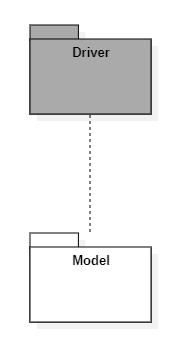
\includegraphics[width=0.2\linewidth]{Impl1.png}
    \caption{Model developing}
\end{figure}
\newpage
\noindent
\textbf{[F1] Sign in and Sign up} \\
The initial functionality to be implemented is the authentication system, encompassing both sign-in and sign-up features, which are respectively managed by the Login Manager and the Registration Manager.

\begin{figure}[H]
    \centering
    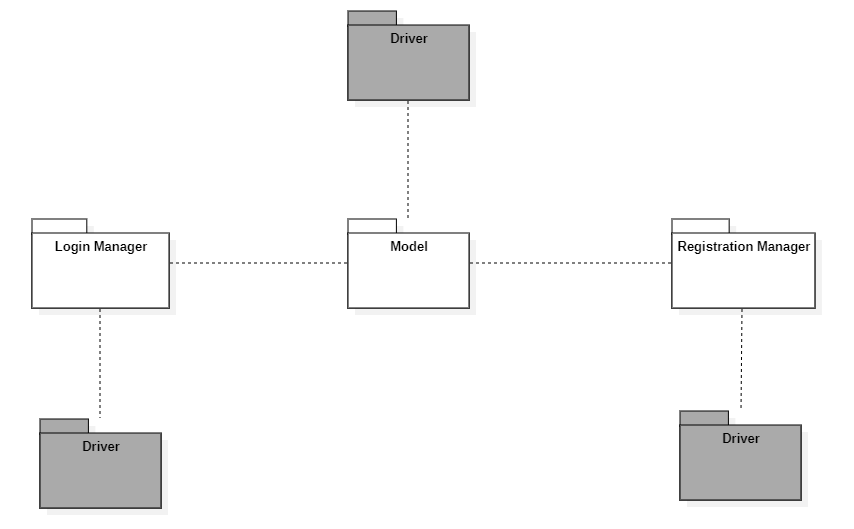
\includegraphics[width=\linewidth]{Impl2.png}
    \caption{Caption}
\end{figure}

\newpage
\noindent
\textbf{[F2] Badge Management} \\
Following the authentication system, the next focus is on constructing the core of the system: the Tournament Manager. The initial step involves the implementation of the Badge Manager, a crucial component required for the tournament creation process.
\begin{figure}[H]
    \centering
    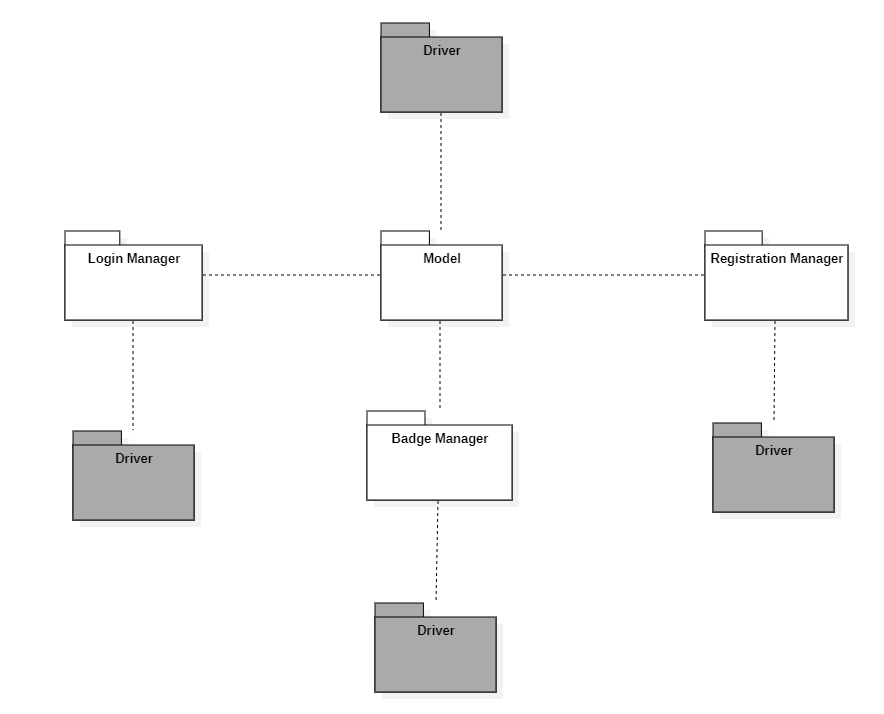
\includegraphics[width=\linewidth]{Impl3.png}
    \caption{Caption}
\end{figure}

\newpage
\noindent
\textbf{[F3] Battle Management} \\
The next component to be implemented is the Battle Manager. This functionality empowers educators to create battles within the tournament. Additionally, it represents the second and final core component required by the Tournament Manager.
\begin{figure}[H]
    \centering
    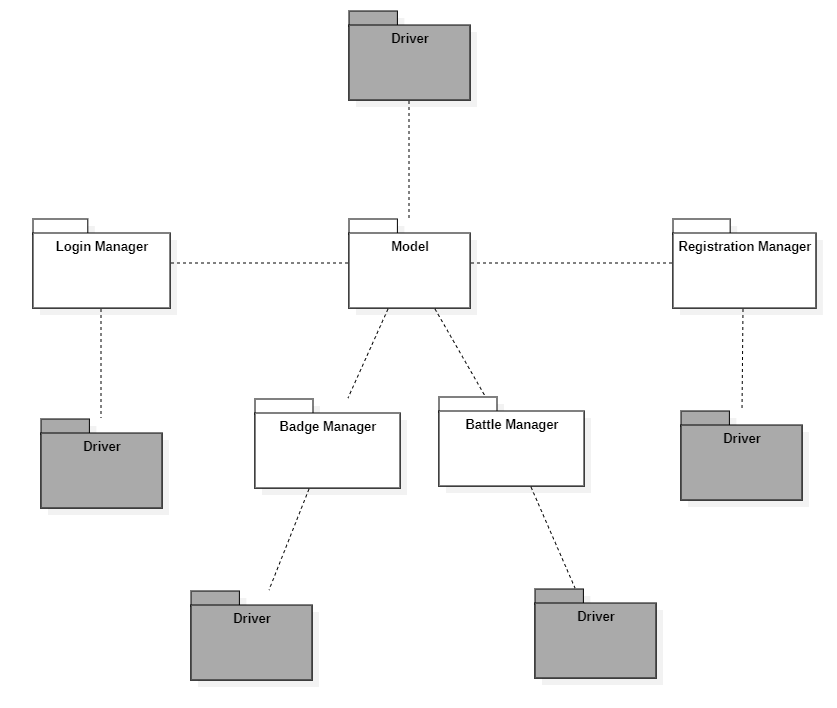
\includegraphics[width=\linewidth]{Impl4.png}
    \caption{Caption}
\end{figure}

\newpage
\noindent
\textbf{[F4] Tournament Management} \\
With both the Badge Manager and Battle Manager now implemented, the subsequent component in line for implementation is the Tournament Manager. This pivotal component empowers users to create, access, and manage tournaments. The implementation is further enhanced by integrating GitHub and CodeScene APIs, although they are not represented in this diagram as they are considered external components.
\begin{figure}[H]
    \centering
    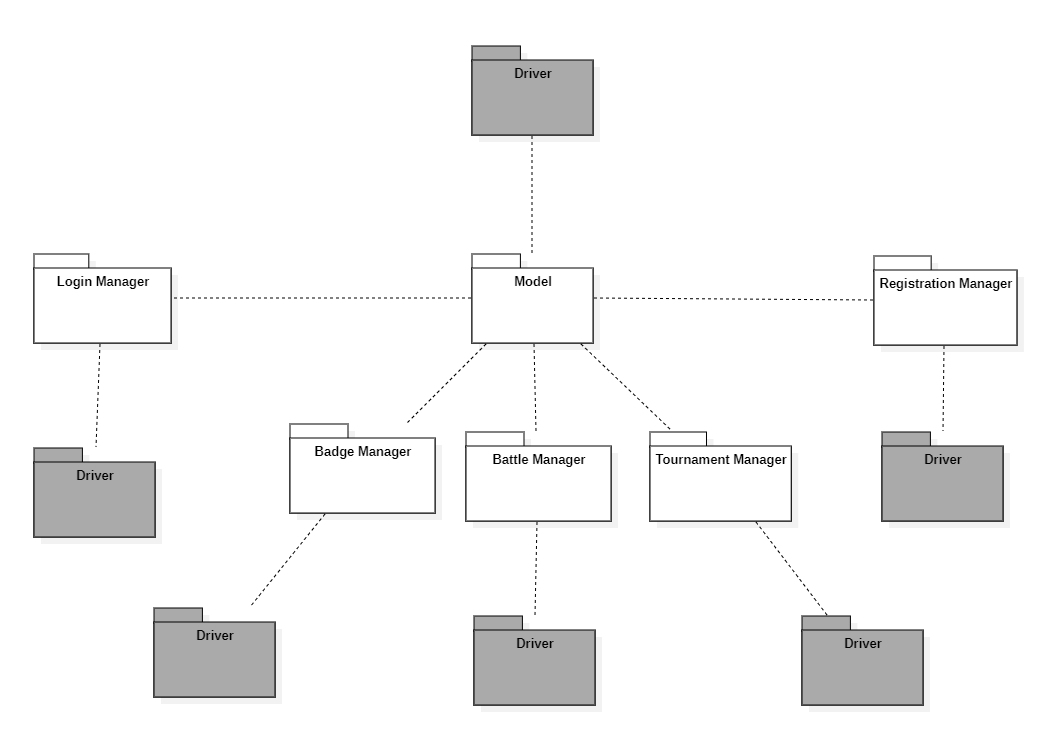
\includegraphics[width=\linewidth]{Impl5.png}
    \caption{Caption}
\end{figure}

\newpage
\noindent
\textbf{[F5] User Notification} \\
After the implementation of both the authentication and tournament systems, the subsequent component to be addressed is the Notification Manager. This integral component facilitates users in receiving various notifications, including invitations to tournaments and battles.
\begin{figure}[H]
    \centering
    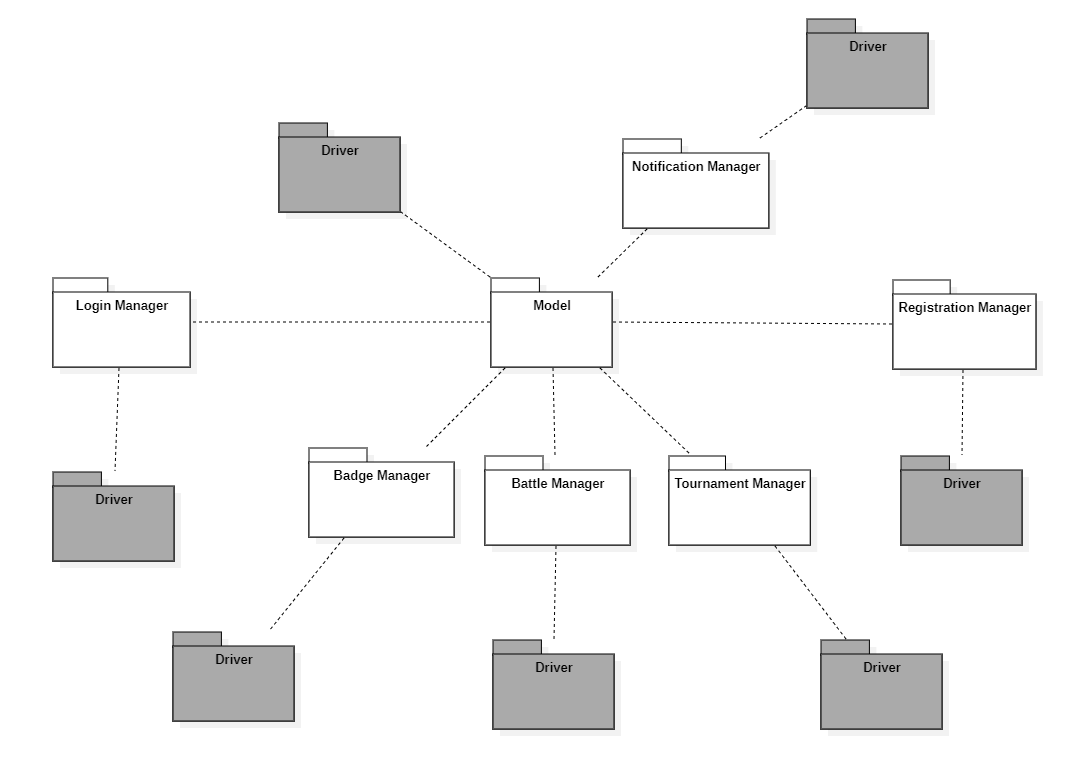
\includegraphics[width=\linewidth]{Impl6.png}
    \caption{Caption}
\end{figure}

\newpage
\noindent
\textbf{[F6] Searching} \\
Lastly, the Search Manager is the final component to be implemented. This component will enable users to search for tournaments and other user profiles.
\begin{figure}[H]
    \centering
    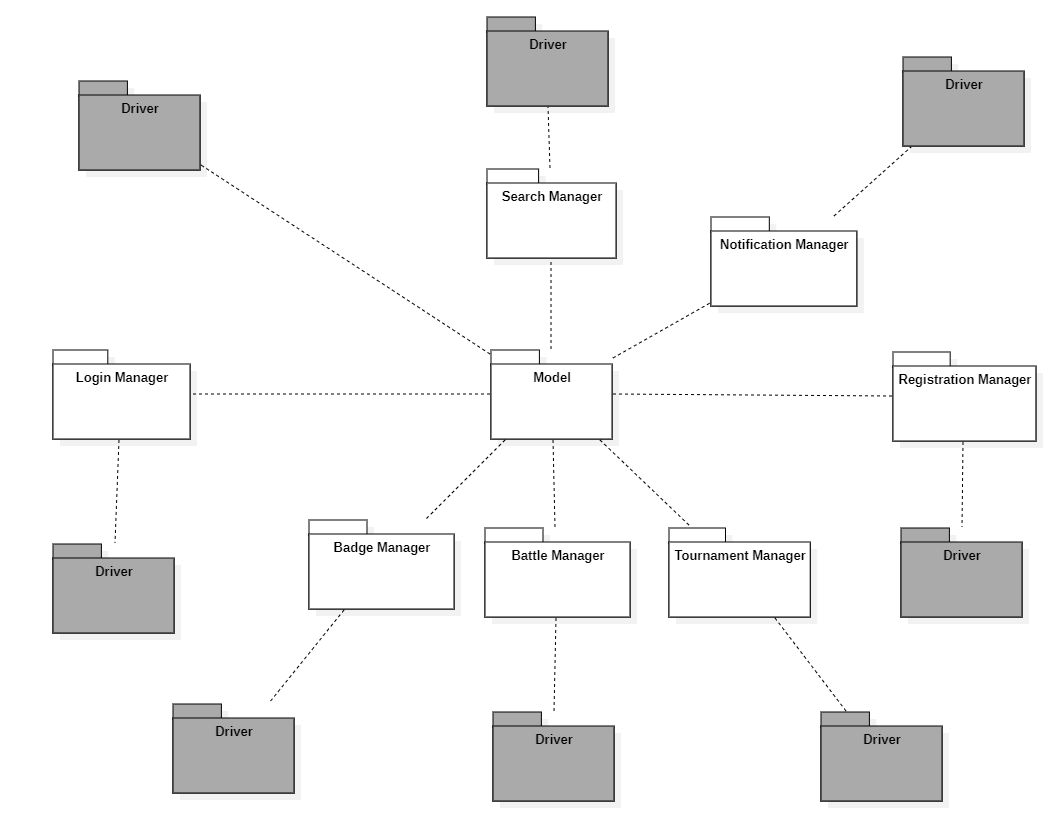
\includegraphics[width=\linewidth]{Impl7.png}
    \caption{Caption}
\end{figure}
\newpage
\subsection{System Testing}
The CKB system needs to be tested to verify the correctness of the behavior of each component, singularly and in their interaction with the other ones.
Each component that is gonna be implemented should be tested singularly (whether possible) and in their integration with the other ones.\\
Once all the components have been implemented and tested it's time to test the whole system to verify it satisfies what is requested in the RASD in a matter of requirements: in this phase, the tested system should be the nearest possible to a final version of the product.
The testing phase could also comprehend beta versions, released to be tested by stakeholders themselves.
The system testing in particular should follow these steps:

\begin{itemize}
    \item \textbf{Functional Testing}: The system should be tested for the ability to satisfy all the requirements described in the RASD in the right manner.
    \item \textbf{Performance Testing}: The system, since not being used for any kind of emergency case, has not very strict performance pretensions: it should be anyway tested to grant the absence of large
    inefficiencies or bottlenecks that could highly affect its usage by the stakeholders.
    This type of test needs a performance quality and workload target to be executed.
    \item \textbf{Usability Testing} : This should be performed to grant the stakeholders can easily use the system, beta versions could be useful to verify the achievement of this target.
    \item \textbf{Load Testing}: It is useful to spot any problems in terms of memory: the test should be executed with the maximum possible memory load for the system to discover any leak, overflow, fault, or memory mismanagement and individuate the limits of the components.
    \item \textbf{Stress Testing}: The system should be tested after being appositely broken (in a recoverable way) to see its capacity to recover after failure.
\end{itemize}
\newpage
\section{Effort Spent}
\begin{center}
\textbf{Armando Fiorini} \\
\vspace{10px} 
    \begin{tabularx}{0.8\textwidth} { 
  | >{\centering\arraybackslash}X 
  | >{\centering\arraybackslash}X | }
 \hline
 \textbf{Chapter} & \textbf{Hours Spent} \\
 \hline
 1 & 1  \\
 \hline
 2 & 23\\
 \hline
 3 & 0\\
 \hline
 4 & 0 \\
 \hline
 5 & 3 \\
 \hline
\end{tabularx}

\vspace{10px}
\textbf{Samuele Motta} \\
\vspace{10px}
\begin{tabularx}{0.8\textwidth} { 
  | >{\centering\arraybackslash}X 
  | >{\centering\arraybackslash}X | }
 \hline
 \textbf{Chapter} & \textbf{Hours Spent} \\
 \hline
 1 & 2  \\
 \hline
 2 & 15 \\
 \hline
 3 & 10 \\
 \hline
 4 & 2 \\
 \hline
 5 & 7 \\
 \hline
\end{tabularx}

\vspace{10px}
\textbf{Vajihe Gholami} \\
\vspace{10px}
\begin{tabularx}{0.8\textwidth} { 
  | >{\centering\arraybackslash}X 
  | >{\centering\arraybackslash}X | }
 \hline
 \textbf{Chapter} & \textbf{Hours Spent} \\
 \hline
 1 & 1  \\
 \hline
 2 & 13 \\
 \hline
 3 & 0 \\
 \hline
 4 & 0 \\
 \hline
 5 & 0 \\
 \hline
\end{tabularx}

\end{center}

\section{References}
\begin{itemize}
    \item Diagrams made with: StarUML and draw.io
    \item Mockups made with: moqups.com
\end{itemize}
\end{document}
